% =====================================================================
%  CO3133 Deep Learning and Its Applications -- Assignment 02 report
%  Group Goat -- Emotion classification on dair-ai/emotion
%  Compile with XeLaTeX or LuaLaTeX (Vietnamese names need Unicode fonts).
%  On Overleaf: Menu -> Compiler -> XeLaTeX.
%  Every number in this file comes from ../results/ (exported by the
%  notebook) or from the run notebook output. Items marked TODO are
%  still missing and must be filled by the group before submission.
% =====================================================================
\documentclass[11pt,a4paper]{article}

\usepackage{iftex}
\ifPDFTeX
  \usepackage[utf8]{inputenc}
  \usepackage[T5]{fontenc}
  \usepackage{lmodern}
\else
  \usepackage{fontspec}
\fi

\usepackage[a4paper,margin=2.4cm,headheight=14pt]{geometry}
\usepackage{amsmath,amssymb,bm}
\usepackage{graphicx}
\usepackage{booktabs,tabularx,multirow,array,makecell}
\usepackage[table]{xcolor}
\usepackage{caption,subcaption}
\usepackage{enumitem}
\usepackage{fancyhdr}
\usepackage{float}
\usepackage{tikz}
\usetikzlibrary{arrows.meta,positioning,fit,calc}
\usepackage[hidelinks]{hyperref}
\usepackage{xurl}

% ---------- colours, links, small helpers ----------
\definecolor{bkblue}{HTML}{1F3A5F}
\definecolor{linkblue}{HTML}{1A6AA8}
\definecolor{lightgray}{HTML}{F2F4F7}
\hypersetup{colorlinks=true,linkcolor=bkblue,urlcolor=linkblue,citecolor=linkblue}
\newcommand{\run}[1]{\texttt{\detokenize{#1}}}          % run identifier (W&B / checkpoint name)
\newcommand{\todo}[1]{\textcolor{red}{\textbf{[TODO: #1]}}}
\newcommand{\pmstd}[2]{#1\,$\pm$\,#2}
\newcolumntype{L}{>{\raggedright\arraybackslash}X}
\newcolumntype{C}{>{\centering\arraybackslash}X}
\setlist{itemsep=2pt,topsep=4pt}
\captionsetup{font=small,labelfont=bf}
\renewcommand{\arraystretch}{1.15}

% ---------- header / footer (same layout as the group's A1 report) ----------
\pagestyle{fancy}
\fancyhf{}
\fancyhead[L]{\small\textcolor{bkblue}{Group Goat --- HCMUT}}
\fancyhead[R]{\small\textcolor{bkblue}{\textbf{CO3133: Deep Learning} --- Assignment 2 (M3 Final)}}
\fancyfoot[L]{\small\textcolor{gray}{Author: Võ Lê Thành Triệu (2453297)}}
\fancyfoot[R]{\small\textbf{Page \thepage}}
\renewcommand{\headrulewidth}{0.4pt}
\renewcommand{\footrulewidth}{0.4pt}
\fancypagestyle{plain}{\fancyhf{}%
  \fancyhead[L]{\small\textcolor{bkblue}{Group Goat --- HCMUT}}%
  \fancyhead[R]{\small\textcolor{bkblue}{\textbf{CO3133: Deep Learning} --- Assignment 2 (M3 Final)}}%
  \fancyfoot[L]{\small\textcolor{gray}{Author: Võ Lê Thành Triệu (2453297)}}%
  \fancyfoot[R]{\small\textbf{Page \thepage}}}

\begin{document}

% =====================================================================
%  TITLE PAGE
% =====================================================================
\begin{center}

\includegraphics[width=0.17\textwidth]{hcmut.png}\par\vspace{0.6cm}
{\Large\scshape Ho Chi Minh City University of Technology (HCMUT) --- VNU-HCM\par}
\vspace{0.15cm}
{\large\scshape Faculty of Computer Science and Engineering\par}
\vspace{0.6cm}
\rule{\textwidth}{1.2pt}\par\vspace{0.3cm}
{\LARGE\bfseries CO3133: Deep Learning and Its Applications\par}
\vspace{0.15cm}
{\Large\bfseries Assignment 02: Deep Learning on Large-Scale Data and Specialized Tasks\par}
\vspace{0.2cm}
{\large\bfseries Text Classification Track --- Six-Class Emotion Recognition on \texttt{dair-ai/emotion}:\\
a TF-IDF Baseline versus Fine-Tuned DistilBERT and BERT\par}
\vspace{0.15cm}
{\normalsize Final Report covering M1 (Proposal), M2 (Draft) and M3 (Final)\par}
\vspace{0.3cm}
\rule{\textwidth}{1.2pt}\par\vspace{0.7cm}

\begin{tabularx}{\textwidth}{@{}>{\bfseries}p{4.1cm}L@{}}
Course Code / Term: & CO3133 --- Semester 261 (Academic Year 2026--2027)\\
Instructor: & Lê Thành Sách\\
Group: & Group Goat\\
Author \& Lead: & \textbf{Võ Lê Thành Triệu} (Student ID \textbf{2453297}) --- 100\% of Assignment 02\\
Other Members: & Hoàng Trọng Huy Minh (2452743, 0\% of A2; Assignment 1), Nguyễn Huỳnh Nam Quốc (2453089, 0\% of A2; Assignment 3)\\
Dataset Proposal: & M1 Dataset Proposal 01 --- status \textbf{Approved}\\
Repository: & \url{https://github.com/volethanhtrieu/DL_Assignment-02}\\
Assignment Page: & \url{https://volethanhtrieu.github.io/DL_Assignment-02/}\\
Experiment Tracking: & \href{https://wandb.ai/trieu-vo1301-ho-chi-minh-city-university-of-technology/goat-a2-emotion}{Weights \& Biases project \texttt{goat-a2-emotion} (public, 12 runs)}\\
Checkpoints: & \href{https://drive.google.com/drive/folders/1WttjY7wrF5sedQDN2Oqnfmd_Hs6dLFk4?usp=drive_link}{Google Drive folder \texttt{DL}} (view only): all 12 checkpoints in \texttt{A2/checkpoints/}; selected DistilBERT + selected baseline also as \texttt{A2/checkpoints\_final.zip} (257.3 MB)\\
Model Hub \& Demo: & \href{https://huggingface.co/TrieuVo/goat-a2-emotion}{Hugging Face model repo \texttt{TrieuVo/goat-a2-emotion}} (selected model + baseline); \href{https://huggingface.co/spaces/TrieuVo/goat-a2-emotion-demo}{live demo Space} (both models run in the browser)\\
Slides: & \href{https://github.com/volethanhtrieu/DL_Assignment-02/blob/main/slides/Goat_A2_Slides.pdf}{\texttt{slides/Goat\_A2\_Slides.pdf}} in the repository\\
Presentation Video: & \href{https://www.youtube.com/watch?v=ok-hF_vicjc}{YouTube: \texttt{youtube.com/watch?v=ok-hF\_vicjc}} (14:48)\\
Submission Date: & 11 November 2026 (M3 Final, due 11 Nov 2026, 23:59 GMT+7)\\
\end{tabularx}

\end{center}
\clearpage
\begin{abstract}
\noindent
We classify short English texts into six emotions (sadness, joy, love, anger, fear, surprise) using the \texttt{split} configuration of \texttt{dair-ai/emotion}, pinned to one Hugging Face revision. A duplicate audit found 51 repeated-text groups with conflicting labels; after the approved filtering rules the splits contain 15,923 / 1,993 / 2,000 texts with no shared text between them. We compare a TF-IDF + logistic regression baseline (CPU) with full fine-tuning of DistilBERT and BERT (Colab T4), each transformer trained with three seeds. All choices (class weights, text cleaning, checkpoint epoch, final model) were made on validation Macro-F1 with rules fixed in advance; the test set was used once.
On test, the selected model, DistilBERT full fine-tune (seed 42), reaches \textbf{accuracy 0.9270 and Macro-F1 0.8902} (three seeds: \pmstd{0.8861}{0.0038}), against 0.8905 / 0.8548 for the best baseline. The gain holds for all six classes and is largest on long texts, texts with ``but'' and negated texts. BERT is statistically tied with DistilBERT (\pmstd{0.8878}{0.0004}; 62 vs.\ 60 texts that only one of the two gets right) at about twice the cost, and a frozen DistilBERT encoder fails under the same recipe (\pmstd{0.4210}{0.0020}). The baseline is about 45$\times$ faster per text on the same CPU. Error analysis shows that most remaining errors sit between close emotions (joy/love, the negative emotions, fear/surprise) and that part of them point to doubtful labels.
\end{abstract}
\vspace{0.6cm}
\tableofcontents
\clearpage

% =====================================================================
\part{Problem and Data}
% =====================================================================

\section{Problem Formulation}

\subsection{Motivation}
Recognising the emotion expressed in a short text is useful for customer-feedback triage, social-media monitoring and mental-health support tools, where people describe how they feel in one or two sentences. The task is harder than sentiment polarity: several emotions share vocabulary (``I feel so lucky to have him'' can be read as joy or love), a single text can contain more than one emotion, and the labels of public datasets are noisy.

\subsection{Input, Output and Formulation}
The \textbf{input} is one English text $x$ (a sequence of words); the \textbf{output} is one label $y \in \mathcal{Y}=\{0{:}\text{sadness},1{:}\text{joy},2{:}\text{love},3{:}\text{anger},4{:}\text{fear},5{:}\text{surprise}\}$. The prediction unit is one text record. Given a training set $\mathcal{D}=\{(x_i,y_i)\}_{i=1}^{N}$, a model $f_\theta$ outputs logits $\mathbf{z}=f_\theta(x)\in\mathbb{R}^{6}$ and class probabilities
\begin{equation}
p_\theta(y=k\mid x)=\frac{\exp(z_k)}{\sum_{j=0}^{5}\exp(z_j)},\qquad \hat{y}=\arg\max_k p_\theta(y=k\mid x).
\end{equation}
Parameters are learned by minimising a class-weighted cross-entropy (Section~\ref{sec:training}). Because the classes are imbalanced, the primary metric is Macro-F1, the unweighted mean of the per-class F1 scores, with accuracy reported alongside it (handbook \S20.1):
\begin{equation}
\text{Macro-F1}=\frac{1}{6}\sum_{c=0}^{5}\frac{2\,P_c R_c}{P_c+R_c},\qquad
\text{Accuracy}=\frac{1}{N}\sum_{i=1}^{N}\mathbb{1}[\hat{y}_i=y_i].
\end{equation}
Accuracy alone would hide failures on the small classes: always predicting \emph{joy} already gives 0.3475 accuracy on test but only 0.0860 Macro-F1.

\subsection{Main Difficulties}
\begin{itemize}
  \item \textbf{Class imbalance:} joy has 9.37 times as many training texts as surprise.
  \item \textbf{Label noise:} identical texts appear with different labels (Section~\ref{sec:dup}); the dataset card describes the annotations as machine-generated.
  \item \textbf{Close classes and negation:} texts are mostly of the form ``i feel \ldots'' followed by an emotion word, so the label often depends on one word, which can be negated or contrasted (``\ldots but \ldots'').
\end{itemize}

\section{Dataset Description}

\begin{table}[H]
\centering
\caption{Dataset specification.}
\label{tab:dataset}
\begin{tabularx}{\textwidth}{@{}p{4.2cm}L@{}}
\toprule
\textbf{Property} & \textbf{Value}\\
\midrule
Name and source & Emotion, \texttt{dair-ai/emotion} on the Hugging Face Hub, configuration \texttt{split} \cite{saravia2018}\\
Version & Revision \texttt{cab853a1dbdf4c42c2b3ef2173804746df8825fe} (pinned in the notebook)\\
License & Listed as ``other''; the dataset card and the authors' repository restrict use to educational and research purposes\\
Labelling & One categorical label per text; the card lists the annotations as machine-generated and the collection process is only partly described\\
Size & 20,000 texts in the official splits: 16,000 train / 2,000 validation / 2,000 test (80/10/10\%)\\
Format & Two fields, \texttt{text} (string) and \texttt{label} (integer 0--5); loaded from the Parquet files of the pinned revision; storage size 1.29~MB as three Parquet files (train 1.03~MB, validation 0.13~MB, test 0.13~MB; 1,287,193 bytes in total) and 2.17~MB once loaded (dataset card of the pinned revision)\\
Validity & No missing, blank or non-string text and no invalid label in any split\\
Known biases & English only; informal first-person texts dominated by ``i feel \ldots''; imbalanced classes; conflicting duplicates (below)\\
\bottomrule
\end{tabularx}
\end{table}

\section{Exploratory Data Analysis}

\subsection{Class Distribution and Imbalance}
Figure~\ref{fig:classdist} shows the label distribution per split. All splits contain all six classes in similar proportions. In the official training split joy is the largest class (5,362 texts, 33.5\%) and surprise the smallest (572, 3.6\%), an imbalance ratio of 9.37. Two consequences guided the design: Macro-F1 is used for every decision, and class weights were tested as an explicit ablation rather than adopted by default (Section~\ref{sec:design}).

\begin{figure}[H]
\centering
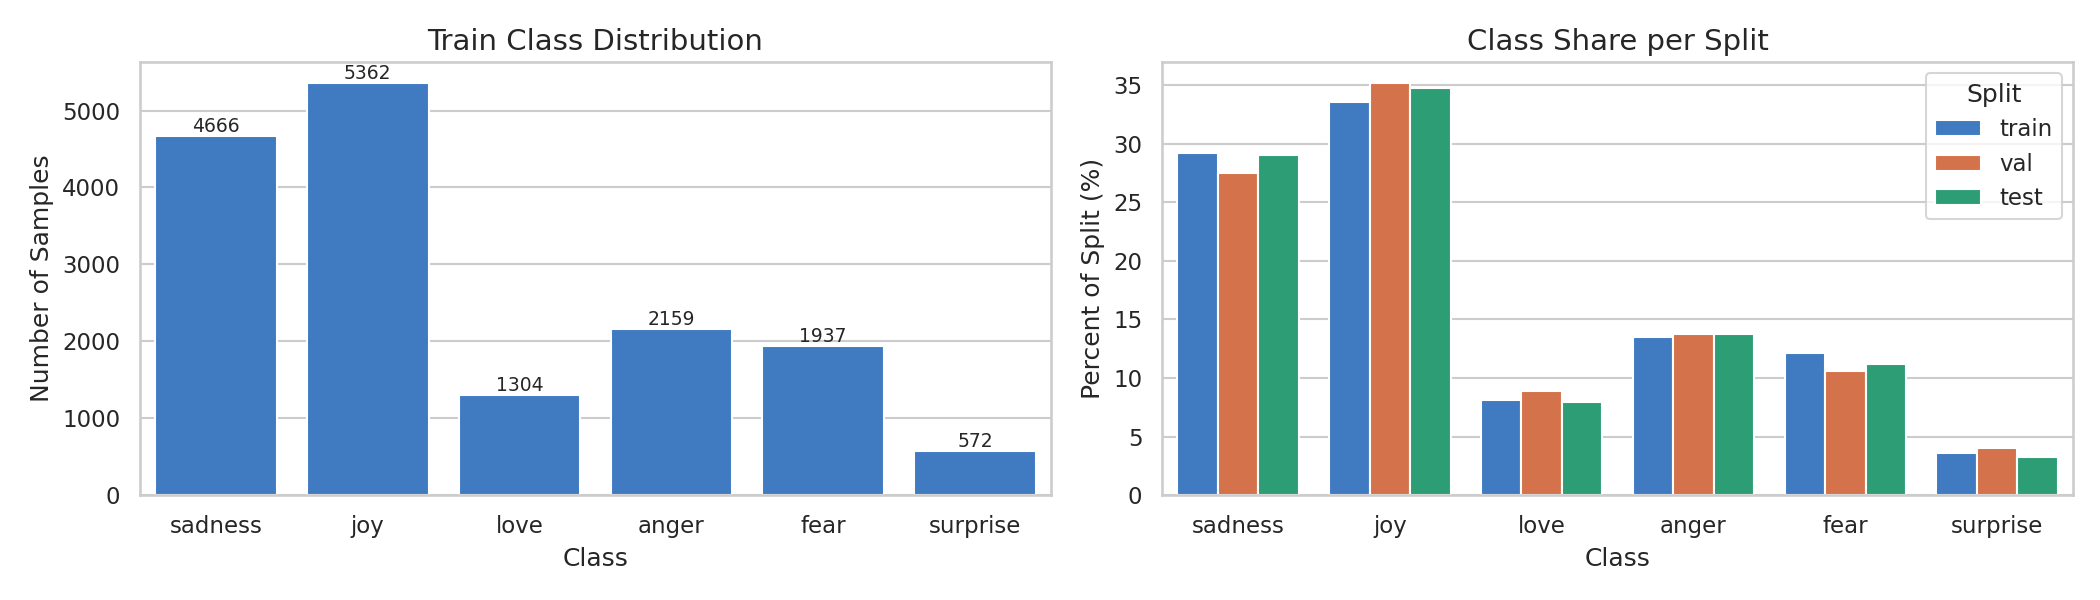
\includegraphics[width=\textwidth]{figures/a2_class_dist.png}
\caption{Class distribution per split (official release, before filtering).}
\label{fig:classdist}
\end{figure}

\subsection{Text Length}
Texts are short. On the official training split the median length is 86 characters / 17 words (mean 96.85 / 19.17, 95th percentile 207 / 41, maximum 300 / 66); the longest validation and test texts have 61 words. Per-class median lengths lie between 16 and 19 words, so length alone does not reveal the class. With the DistilBERT WordPiece tokenizer (Section~\ref{sec:prep}) a text has a median of 20 tokens including \texttt{[CLS]} and \texttt{[SEP]}, a 95th percentile of 45, a 99th percentile of 57 and a maximum of 87 (train), 69 (val) and 66 (test); there are 1.06 tokens per word. No text exceeds 128 tokens, so the planned maximum length of 128 never truncates.

\begin{figure}[H]
\centering
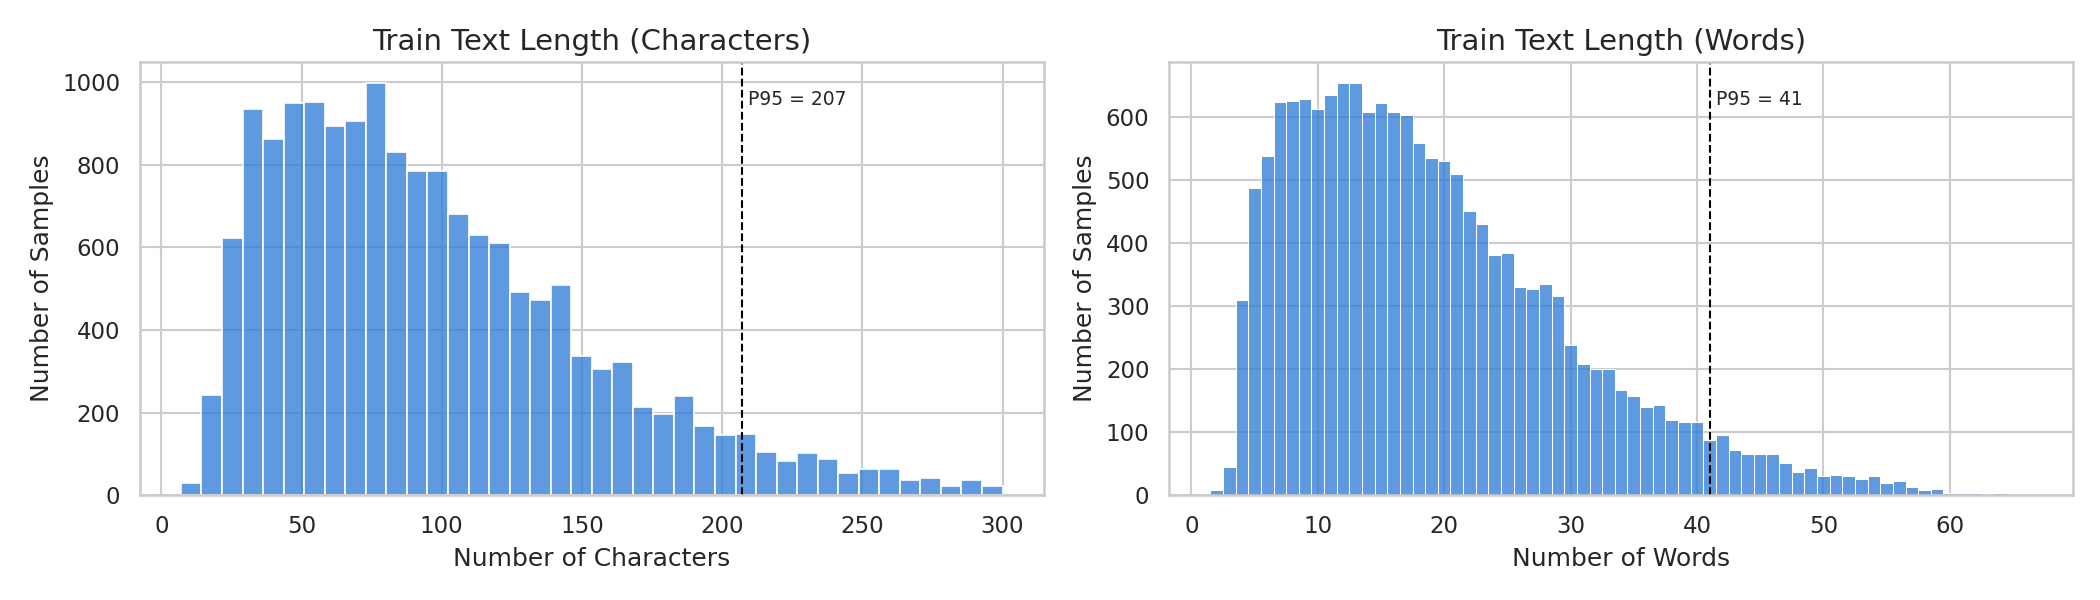
\includegraphics[width=\textwidth]{figures/a2_text_len.png}
\caption{Distribution of text length per split.}
\label{fig:textlen}
\end{figure}

\subsection{Duplicates and Conflicting Labels}
\label{sec:dup}
Texts were compared after a normalisation of Unicode NFC, lowercasing, trimming and collapsing whitespace; exact and normalised comparison gave the same groups (Table~\ref{tab:dup}). Over all 20,000 texts there are 52 repeated-text groups, and \textbf{51 of them carry conflicting labels} (102 rows, two per group). Fourteen of the conflicting groups include a test text. These rows show two problems: \emph{leakage} (the same text in two splits) and \emph{label noise} (the same text with two emotions).

\begin{table}[H]
\centering
\caption{Repeated or shared text groups (official release).}
\label{tab:dup}
\begin{tabular}{@{}lr@{\hspace{2.2em}}lr@{}}
\toprule
\textbf{Scope} & \textbf{Groups} & \textbf{Scope} & \textbf{Groups}\\
\midrule
Within train & 31 & Train--validation overlap & 5\\
Within validation & 2 & Train--test overlap & 11\\
Within test & 0 & Validation--test overlap & 3\\
\bottomrule
\end{tabular}
\end{table}

\subsection{Vocabulary and Class-Specific Words}
The training vocabulary (minimal cleaning) has 15,188 word types; 51.5\% of them occur only once, and 2.72\% / 2.74\% of the validation / test tokens are not in the training vocabulary. ``feel'' occurs in 66.4\% of training texts and ``feeling'' in 31.1\%. The most class-specific n-grams are the emotion adjectives themselves (Figure~\ref{fig:ngrams}; e.g.\ \emph{offended}, \emph{intimidated}, \emph{amazed}), many of which appear in a single class only. This suggested that the labels largely follow one emotion word, a hypothesis that the error analysis later tests.

\begin{figure}[H]
\centering
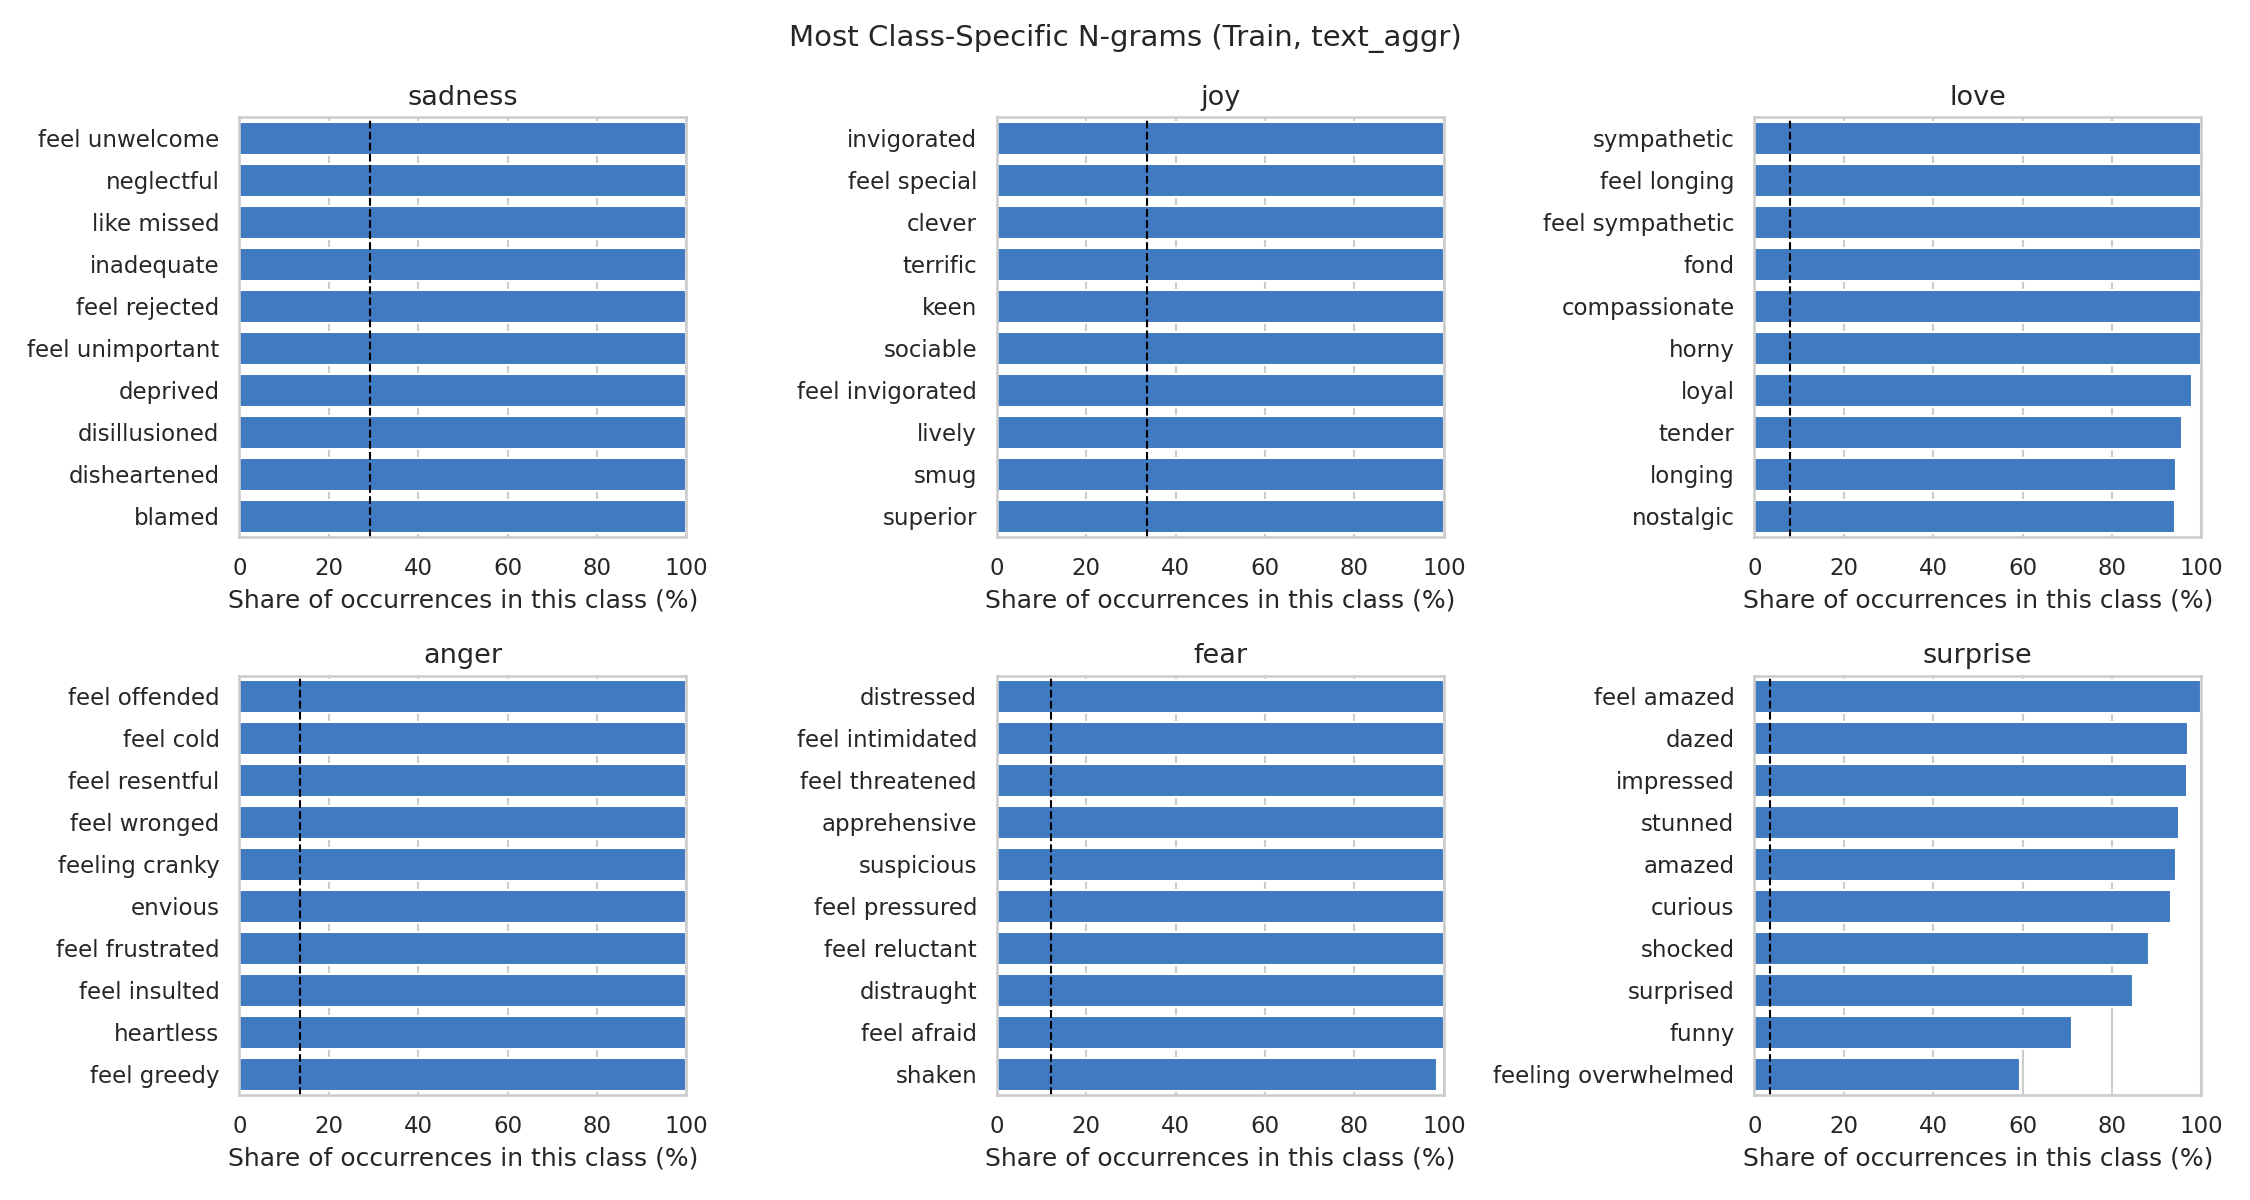
\includegraphics[width=0.92\textwidth]{figures/a2_top_ngrams.png}
\caption{Most frequent and most class-specific n-grams per class (training split, stopwords removed).}
\label{fig:ngrams}
\end{figure}

\section{Data Splitting and Leakage Prevention}
\label{sec:split}
The official train/validation/test splits are kept (no re-splitting, no stratification needed, seed 42 for everything random). The split unit is a \emph{group of texts with the same normalised text}: such a group may not cross splits. The four filtering rules approved in the proposal were applied in order:
\begin{enumerate}
  \item keep the test set unchanged, including its released labels, and remove every training or validation text that also occurs in test;
  \item for remaining train--validation overlaps, keep the validation copy and remove the training copy;
  \item inside each of train and validation, remove every group with conflicting labels (no label is chosen or invented);
  \item for same-label duplicates, keep the first occurrence.
\end{enumerate}

\begin{table}[H]
\centering
\caption{Rows removed by rule and final split sizes.}
\label{tab:filter}
\begin{tabular}{@{}lrrr@{}}
\toprule
\textbf{Reason} & \textbf{Train} & \textbf{Validation} & \textbf{Test}\\
\midrule
Text also in test (rule 1) & 11 & 3 & 0\\
Text also in validation (rule 2) & 5 & -- & --\\
Conflicting-label group (rule 3) & 60 (30 groups) & 4 (2 groups) & 0\\
Same-label duplicate (rule 4) & 1 & 0 & 0\\
\midrule
\textbf{Removed} & \textbf{77} & \textbf{7} & \textbf{0}\\
\textbf{Final size} & \textbf{15,923 (79.95\%)} & \textbf{1,993 (10.01\%)} & \textbf{2,000 (10.04\%)}\\
\bottomrule
\end{tabular}
\end{table}

Seven checks pass after filtering: no shared normalised text between any two splits, no repeated text inside a split, at least 5,000 training texts and all six classes in every split. The class proportions stay close to the original (train: joy 33.54\%, sadness 29.27\%, anger 13.52\%, fear 12.08\%, love 8.06\%, surprise 3.54\%). Everything learned from data (TF-IDF vocabulary and IDF, class weights) is fitted on the training split only. One limitation remains: the five train--validation overlaps all had conflicting labels, so the kept validation copies and the 14 test texts that had a copy elsewhere carry disputed labels.

\section{Preprocessing}
\label{sec:prep}
\begin{itemize}
  \item \textbf{Minimal text} (used by all transformers and two baselines): Unicode NFC, lowercase, single spaces. Stopwords are kept because transformers use them as context. The released texts contain no apostrophes, so ``I'm'' appears as \emph{im} and ``don't'' as \emph{dont} or \emph{don t}.
  \item \textbf{Aggressive text} (one baseline variant): minimal text, then only letters, digits and spaces are kept and the 318 scikit-learn English stopwords are removed \emph{except} 23 negation and intensity words (not, no, never, nothing, without, very, so, too, more, most, but, \ldots). The average training text drops from 19.18 to 9.31 tokens, and no text becomes empty.
  \item \textbf{Tokenisation for transformers:} the model's own uncased WordPiece tokenizer adds \texttt{[CLS]} and \texttt{[SEP]}; truncation at 128 tokens (never reached); padding \emph{per batch} to the longest text of the batch. Padded positions get attention mask 0, so they do not change the predictions. Per-batch padding needs only 36.1\% of the tokens that padding everything to 128 would need on the validation set. BERT and DistilBERT produce identical token ids on all three splits, so both use the same data loaders.
  \item \textbf{Labels:} kept as integers 0--5 with the mapping above. No augmentation is used.
\end{itemize}

\paragraph{One example batch after preprocessing.} The first validation batch has the shapes below (batch size 16; the longest text in it has 34 tokens, so 52.8\% of the batch is padding):

\begin{table}[H]
\centering
\caption{Tensors of one validation batch and one decoded text from it.}
\label{tab:batch}
\begin{tabularx}{\textwidth}{@{}p{3.2cm}p{3.0cm}L@{}}
\toprule
\textbf{Tensor} & \textbf{Shape / type} & \textbf{Content}\\
\midrule
input ids & $(16, 34)$, int64 & WordPiece ids, one row per text\\
attention mask & $(16, 34)$, int64 & 1 for real tokens, 0 for padding\\
labels & $(16,)$, int64 & class ids, equal to the validation labels\\
model output & $(16, 6)$ & one logit per class\\
\midrule
Example text & \multicolumn{2}{L}{``im feeling quite sad and sorry for myself but ill snap out of it soon'' (label 0, sadness)}\\
Tokens & \multicolumn{2}{L}{[CLS] im feeling quite sad \ldots{} soon [SEP] followed by 17 $\times$ [PAD]}\\
\bottomrule
\end{tabularx}
\end{table}

% =====================================================================
\part{Methodology}
% =====================================================================

\section{Pipeline Overview}
Figure~\ref{fig:pipeline} shows the end-to-end pipeline. The two model families share the data, the splits, the filtering and the evaluation; they differ in representation and training.

\begin{figure}[H]
\centering
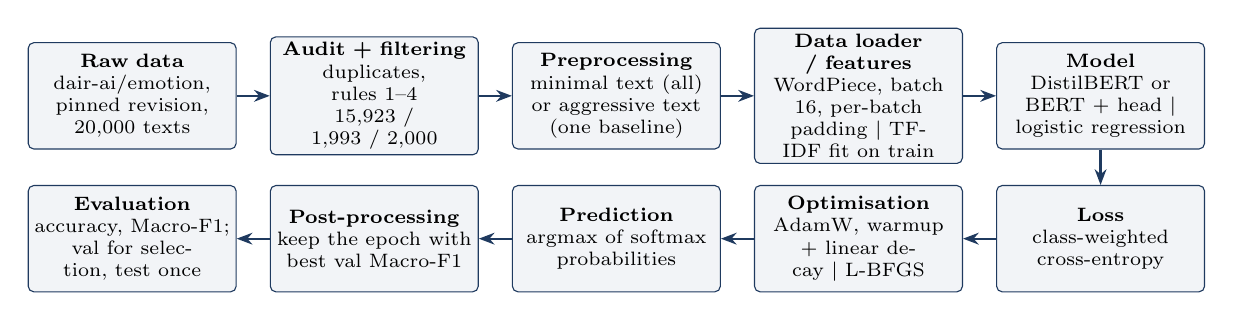
\begin{tikzpicture}[
  node distance=0.45cm and 0.42cm,
  box/.style={draw=bkblue,rounded corners=2pt,fill=lightgray,align=center,font=\scriptsize,text width=2.5cm,minimum height=1.35cm,inner sep=2pt},
  arr/.style={-{Stealth[length=2mm]},thick,bkblue}]
\node[box] (raw) {\textbf{Raw data}\\ dair-ai/emotion, pinned revision, 20,000 texts};
\node[box,right=of raw] (audit) {\textbf{Audit + filtering}\\ duplicates, rules 1--4\\ 15,923 / 1,993 / 2,000};
\node[box,right=of audit] (prep) {\textbf{Preprocessing}\\ minimal text (all) or aggressive text (one baseline)};
\node[box,right=of prep] (load) {\textbf{Data loader / features}\\ WordPiece, batch 16, per-batch padding \textbar{} TF-IDF fit on train};
\node[box,right=of load] (model) {\textbf{Model}\\ DistilBERT or BERT + head \textbar{} logistic regression};
\node[box,below=of model] (loss) {\textbf{Loss}\\ class-weighted cross-entropy};
\node[box,left=of loss] (opt) {\textbf{Optimisation}\\ AdamW, warmup + linear decay \textbar{} L-BFGS};
\node[box,left=of opt] (pred) {\textbf{Prediction}\\ argmax of softmax probabilities};
\node[box,left=of pred] (post) {\textbf{Post-processing}\\ keep the epoch with best val Macro-F1};
\node[box,left=of post] (eval) {\textbf{Evaluation}\\ accuracy, Macro-F1; val for selection, test once};
\draw[arr] (raw) -- (audit);
\draw[arr] (audit) -- (prep);
\draw[arr] (prep) -- (load);
\draw[arr] (load) -- (model);
\draw[arr] (model) -- (loss);
\draw[arr] (loss) -- (opt);
\draw[arr] (opt) -- (pred);
\draw[arr] (pred) -- (post);
\draw[arr] (post) -- (eval);
\end{tikzpicture}
\caption{End-to-end pipeline in the form required by the handbook (read the second row from right to left). Where a box has two parts, the left part is the transformer path and the part after the bar is the baseline path. The only post-processing is keeping the best epoch of each transformer run.}
\label{fig:pipeline}
\end{figure}

\section{Models}
\label{sec:models}

\subsection{Baseline: TF-IDF + Logistic Regression}
The baseline is a classical bag-of-n-grams classifier \cite{salton1988,pedregosa2011}. It has two stages, a TF-IDF feature extractor and a logistic-regression classifier. Both are \emph{fitted on the training split only} and then applied unchanged to validation and test, so no information from those splits enters the features (Figure~\ref{fig:tfidf}).

\begin{figure}[H]
\centering
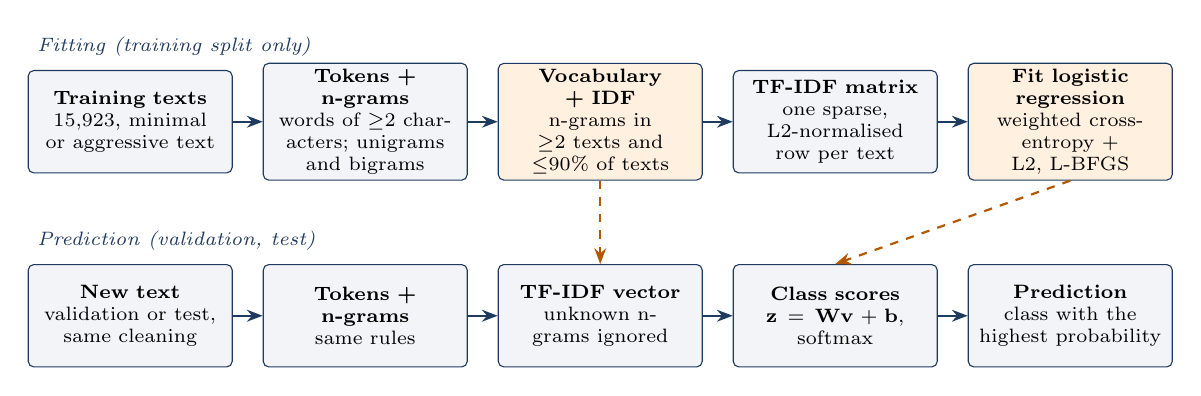
\begin{tikzpicture}[
  node distance=0.5cm and 0.38cm,
  box/.style={draw=bkblue,rounded corners=2pt,fill=lightgray,align=center,font=\scriptsize,text width=2.45cm,minimum height=1.3cm,inner sep=2pt},
  fit/.style={box,fill=orange!12},
  lab/.style={font=\scriptsize\itshape,text=bkblue,anchor=south west},
  arr/.style={-{Stealth[length=2mm]},thick,bkblue},
  dep/.style={-{Stealth[length=2mm]},thick,dashed,orange!70!black}]
% fitting row
\node[box] (t1) {\textbf{Training texts}\\ 15,923, minimal or aggressive text};
\node[box,right=of t1] (n1) {\textbf{Tokens + n-grams}\\ words of $\geq$2 characters; unigrams and bigrams};
\node[fit,right=of n1] (v1) {\textbf{Vocabulary + IDF}\\ n-grams in $\geq$2 texts and $\leq$90\% of texts};
\node[box,right=of v1] (x1) {\textbf{TF-IDF matrix}\\ one sparse, L2-normalised row per text};
\node[fit,right=of x1] (m1) {\textbf{Fit logistic regression}\\ weighted cross-entropy + L2, L-BFGS};
% applying row
\node[box,below=1.15cm of t1] (t2) {\textbf{New text}\\ validation or test, same cleaning};
\node[box,right=of t2] (n2) {\textbf{Tokens + n-grams}\\ same rules};
\node[box,right=of n2] (x2) {\textbf{TF-IDF vector}\\ unknown n-grams ignored};
\node[box,right=of x2] (s2) {\textbf{Class scores}\\ $\mathbf{z}=\mathbf{W}\mathbf{v}+\mathbf{b}$, softmax};
\node[box,right=of s2] (p2) {\textbf{Prediction}\\ class with the highest probability};
\node[lab] at ($(t1.north west)+(0,0.05)$) {Fitting (training split only)};
\node[lab] at ($(t2.north west)+(0,0.05)$) {Prediction (validation, test)};
\draw[arr] (t1) -- (n1); \draw[arr] (n1) -- (v1); \draw[arr] (v1) -- (x1); \draw[arr] (x1) -- (m1);
\draw[arr] (t2) -- (n2); \draw[arr] (n2) -- (x2); \draw[arr] (x2) -- (s2); \draw[arr] (s2) -- (p2);
\draw[dep] (v1.south) -- (x2.north);
\draw[dep] (m1.south) -- (s2.north);
\end{tikzpicture}
\caption{TF-IDF + logistic-regression pipeline. Orange boxes are the only learned parts; dashed arrows show that validation and test texts reuse the vocabulary, IDF weights and classifier learned from the training split.}
\label{fig:tfidf}
\end{figure}

\paragraph{Stage 1: TF-IDF features.}
\begin{enumerate}[leftmargin=*,itemsep=1pt]
  \item \emph{Tokens and n-grams.} The cleaned text is split into words of at least two letters or digits (the library default), so the pronoun ``i'', present in 93.2\% of training texts, is not a feature. Every word (unigram) and every pair of adjacent words (bigram) is a candidate feature; bigrams keep a little word order, e.g.\ ``not happy'' differs from ``happy''.
  \item \emph{Vocabulary.} Only n-grams that occur in at least 2 training texts (this removes typos and one-off phrases) and in at most 90\% of them (this removes near-universal terms) are kept: 32,776 n-grams with minimal text and 17,070 with aggressive text. Each kept n-gram is one dimension of the feature vector.
  \item \emph{Weighting.} The weight of n-gram $t$ in text $d$ is
  \begin{equation}
  \text{tfidf}(t,d)=\text{tf}(t,d)\cdot\Big(\ln\frac{1+n}{1+\text{df}(t)}+1\Big),
  \end{equation}
  where $\text{tf}(t,d)$ is the count of $t$ in $d$, $n$ the number of training texts and $\text{df}(t)$ the number of training texts that contain $t$. An n-gram that is frequent in the text but rare in the corpus (an emotion adjective) gets a large weight; a common one (``feel'', in 66.4\% of texts) a small one.
  \item \emph{Normalisation.} Each vector is divided by its L2 norm, so long and short texts are on the same scale. Almost all entries are zero, because a text contains only a few of the thousands of n-grams.
\end{enumerate}
For example, the training text ``i do not feel reassured anxiety is on each side'' (label joy) becomes ``not feel reassured anxiety'' after aggressive cleaning; its candidate features are the unigrams \emph{not, feel, reassured, anxiety} and the bigrams \emph{not feel, feel reassured, reassured anxiety}. Those in the vocabulary receive a TF-IDF weight; every other dimension is zero.

\paragraph{Stage 2: logistic regression.}
A multinomial logistic regression maps the vector $\mathbf{v}\in\mathbb{R}^{F}$ ($F$ = vocabulary size) to six class scores and probabilities,
\begin{equation}
\mathbf{z}=\mathbf{W}\mathbf{v}+\mathbf{b},\qquad p(y=k\mid\mathbf{v})=\frac{\exp z_k}{\sum_{j=1}^{6}\exp z_j},\qquad \mathbf{W}\in\mathbb{R}^{6\times F},
\end{equation}
so each weight $W_{k,t}$ says how strongly n-gram $t$ pushes a text towards class $k$. Training minimises the class-weighted cross-entropy plus an L2 penalty,
\begin{equation}
\min_{\mathbf{W},\mathbf{b}}\ \tfrac12\lVert\mathbf{W}\rVert^2 + C\sum_{i=1}^{N} w_{y_i}\big(-\log p(y_i\mid\mathbf{v}_i)\big),\qquad w_c=\frac{N}{6N_c},\quad C=1,
\end{equation}
with the L-BFGS optimiser (at most 1,000 iterations). The balanced weights $w_c$ make each class contribute equally to the loss although, after filtering, joy has 5,340 training texts and surprise only 564. The prediction is the class with the highest probability. The model has $6\times(F+1)$ parameters: 196,662 with minimal text and 102,426 with aggressive text.

\paragraph{Variants and role.}
Two text inputs are compared (Section~\ref{sec:prep}): minimal text, and aggressive text that also removes 295 stopwords while keeping negations and intensifiers. Class weights on vs.\ off is a further ablation. The selected baseline (aggressive text, class weights) was chosen on validation (experiment E3). The baseline answers one question: how far do word and word-pair cues alone go on this dataset? \emph{Strengths:} trains in seconds on one CPU core and is fully interpretable, since the largest weights of each class can be read directly (Figure~\ref{fig:features}). \emph{Limits:} no word order beyond bigrams, no notion of negation scope, and no knowledge of words unseen in training.

\begin{figure}[H]
\centering
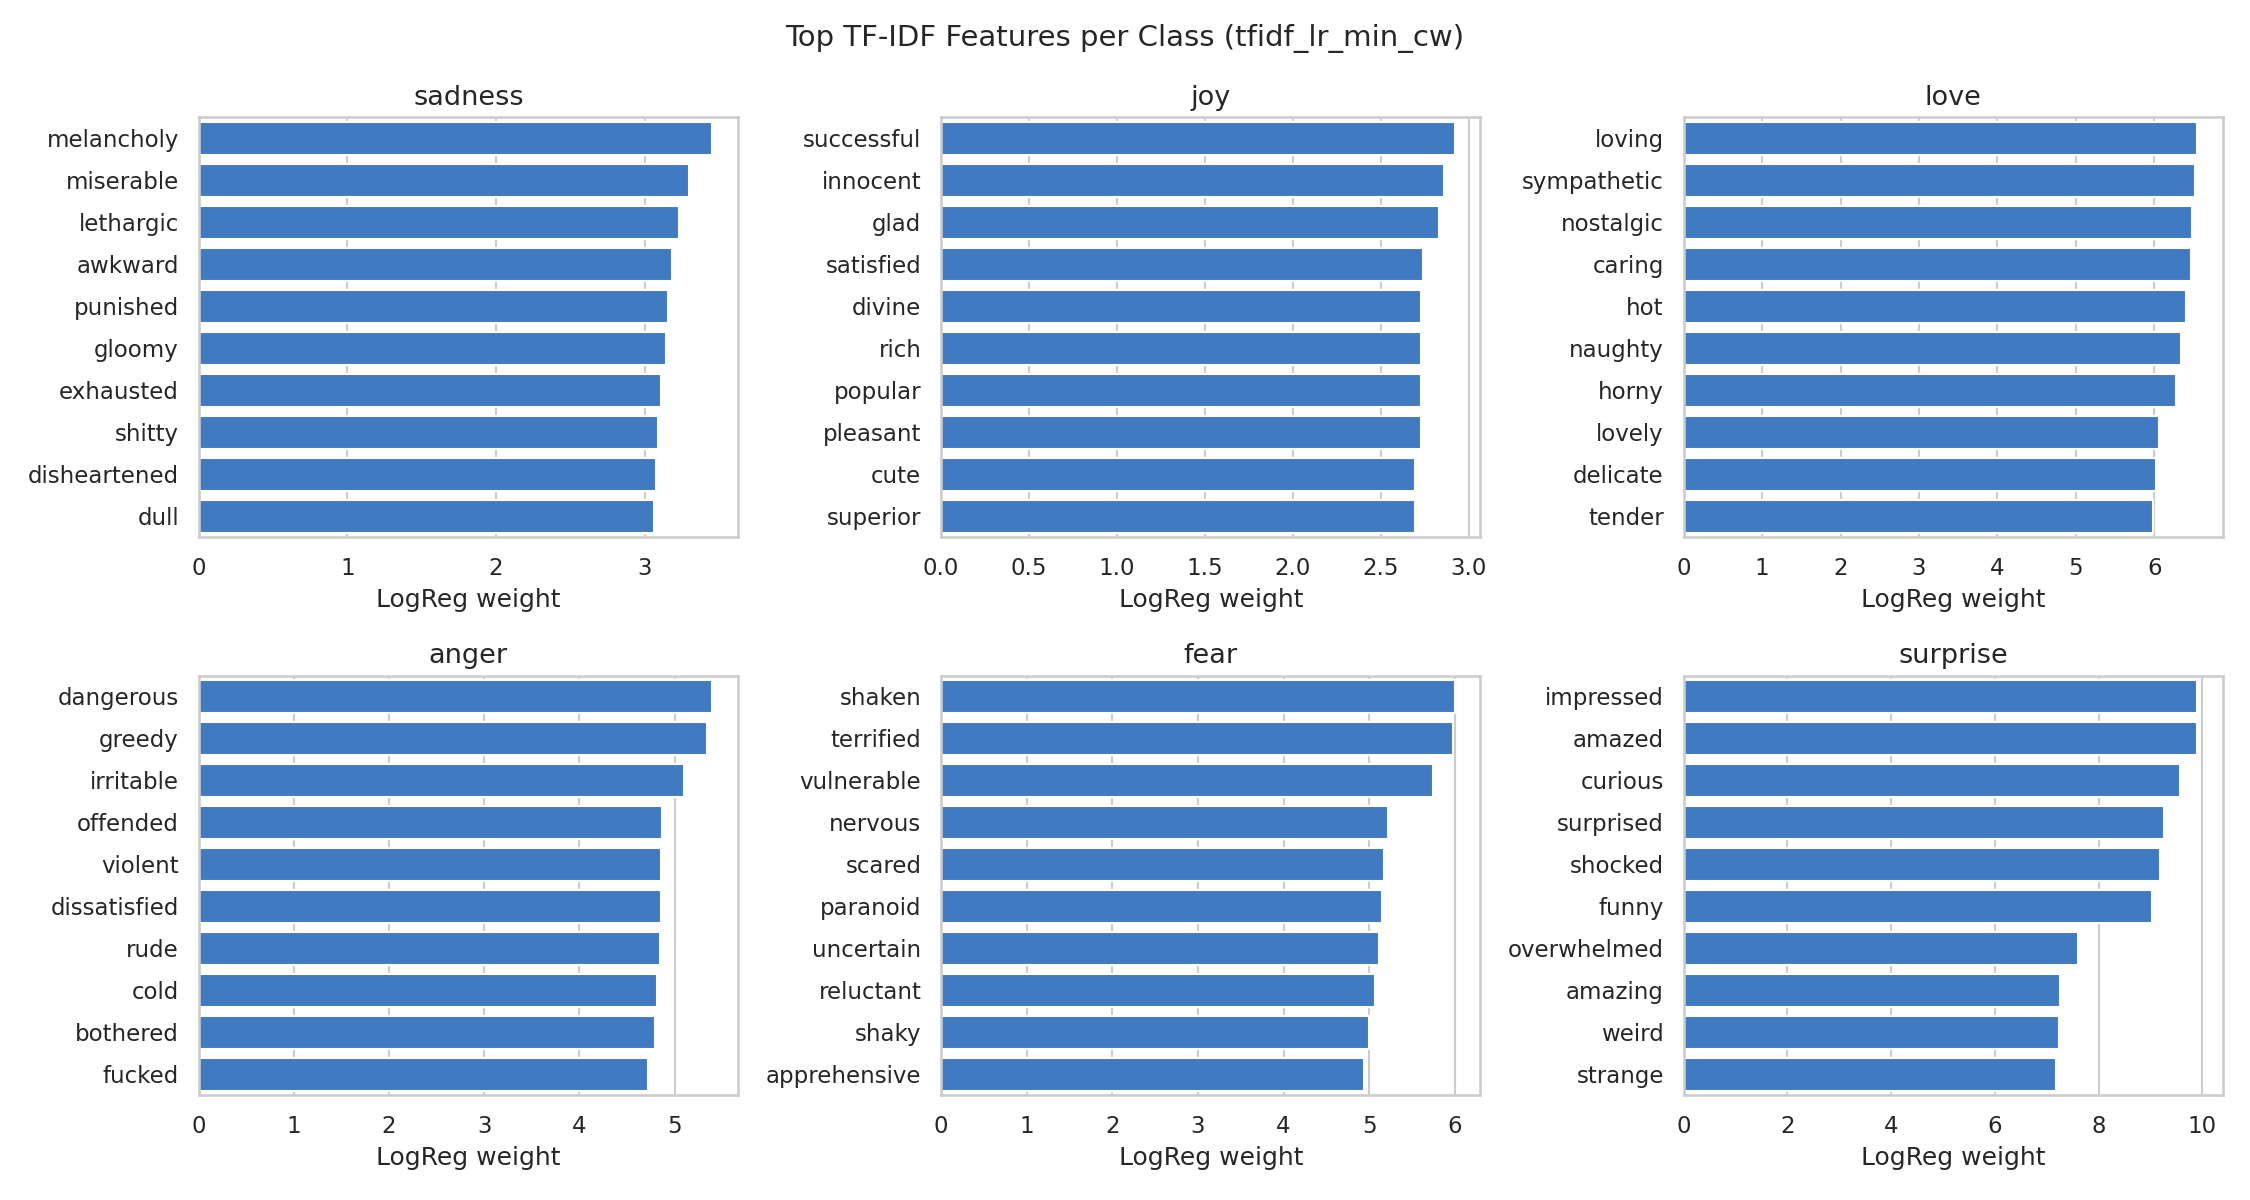
\includegraphics[width=0.92\textwidth]{figures/a2_top_features_tfidf.png}
\caption{Largest logistic-regression weights per class (baseline with class weights, minimal text). The top features are single emotion adjectives.}
\label{fig:features}
\end{figure}

\subsection{Main Model: DistilBERT, Full Fine-Tuning}
DistilBERT (\texttt{distilbert-base-uncased}) \cite{sanh2019} is a 6-layer Transformer encoder (hidden size 768, 12 attention heads) distilled from BERT. The final hidden state of \texttt{[CLS]}, $\mathbf{h}\in\mathbb{R}^{768}$, goes through the standard sequence-classification head:
\begin{equation}
\mathbf{z}=\mathbf{W}_2\,\mathrm{Dropout}\big(\mathrm{ReLU}(\mathbf{W}_1\mathbf{h}+\mathbf{b}_1)\big)+\mathbf{b}_2,\qquad \mathbf{W}_1\in\mathbb{R}^{768\times768},\ \mathbf{W}_2\in\mathbb{R}^{6\times768}.
\end{equation}
The encoder has 66,362,880 parameters and the new head 595,206 (590,592 + 4,614), 66,958,086 in total. In full fine-tuning every parameter is updated. \emph{Strengths:} contextual representations that can model negation and contrast. \emph{Limits:} about 45$\times$ slower than the baseline per text on CPU and needs a GPU to train in minutes.

\subsection{Second Pretrained Model: BERT, Full Fine-Tuning}
BERT (\texttt{bert-base-uncased}) \cite{devlin2019} has 12 layers of the same width. Its classification head is a single linear layer (4,614 parameters) on top of the \emph{pretrained} pooler (a dense layer with tanh on \texttt{[CLS]}), so 109,482,240 of its 109,486,854 parameters are pretrained. BERT was added after the proposal (plan update of 27 Oct 2026, recorded in the repository README) because time remained: it uses exactly the same recipe as DistilBERT, to see what a larger model changes in quality and cost.

Figure~\ref{fig:arch} compares the two architectures. Both read the same WordPiece token ids (checked to be identical on every split) and differ in depth and in the classification head.

\begin{figure}[H]
\centering
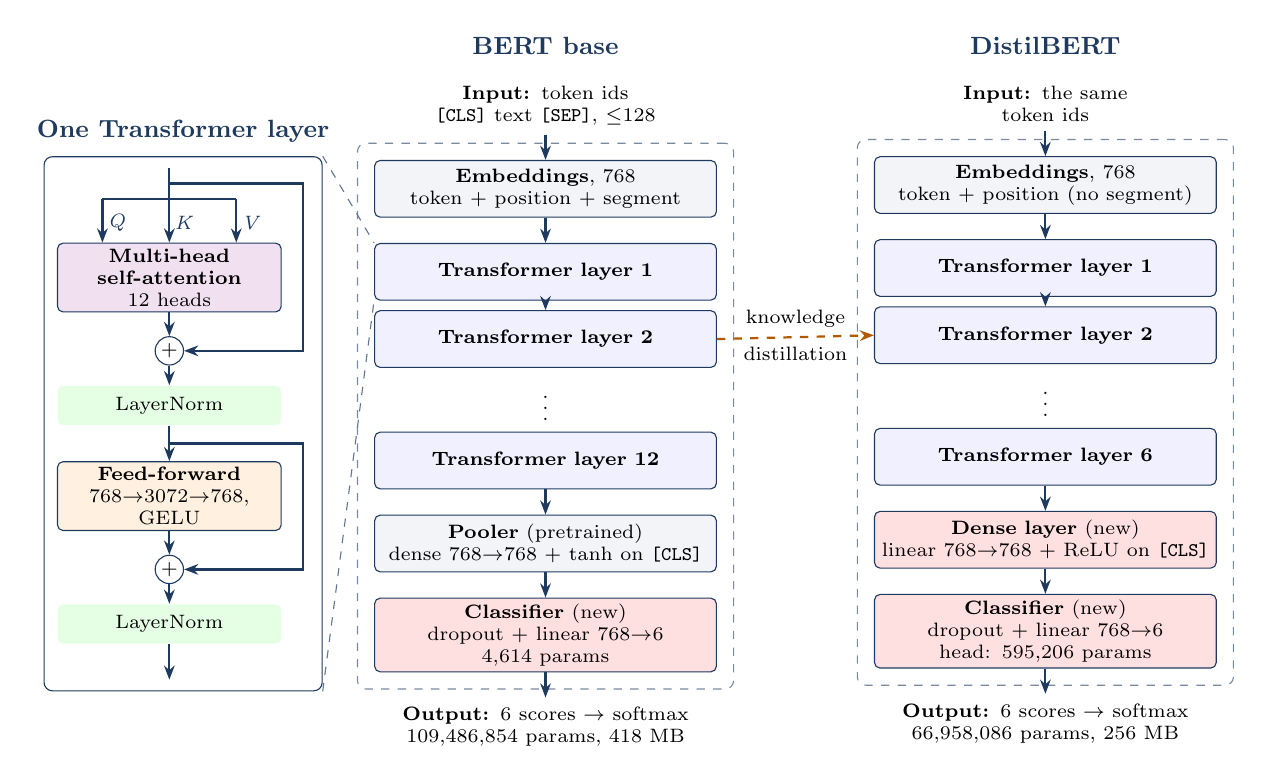
\begin{tikzpicture}[
  node distance=0.32cm,
  pre/.style={draw=bkblue,rounded corners=2pt,fill=lightgray,align=center,font=\scriptsize,text width=4.2cm,minimum height=0.72cm,inner sep=2pt},
  layer/.style={pre,fill=blue!6},
  new/.style={pre,fill=red!12},
  io/.style={align=center,font=\scriptsize,text width=4.2cm},
  arr/.style={-{Stealth[length=1.8mm]},thick,bkblue},
  frame/.style={draw=bkblue!60,dashed,rounded corners=3pt,inner sep=6pt},
  sub/.style={draw=bkblue,rounded corners=2pt,align=center,font=\scriptsize,text width=2.7cm,minimum height=0.62cm,inner sep=2pt},
  norm/.style={sub,draw=none,fill=green!10,minimum height=0.5cm},
  plus/.style={draw=bkblue,circle,inner sep=0pt,minimum size=0.36cm,font=\scriptsize}]
% BERT column
\node[io,font=\small\bfseries,text=bkblue] (bname) {BERT base};
\node[io,below=0.15cm of bname] (bin) {\textbf{Input:} token ids\\ \texttt{[CLS]} text \texttt{[SEP]}, $\leq$128};
\node[pre,below=of bin] (bemb) {\textbf{Embeddings}, 768\\ token + position + segment};
\node[layer,below=of bemb] (bl1) {\textbf{Transformer layer 1}};
\node[layer,below=0.12cm of bl1] (bl2) {\textbf{Transformer layer 2}};
\node[io,below=0.02cm of bl2] (bdots) {$\vdots$};
\node[layer,below=0.02cm of bdots] (bl12) {\textbf{Transformer layer 12}};
\node[pre,below=of bl12] (bpool) {\textbf{Pooler} (pretrained)\\ dense 768$\to$768 + tanh on \texttt{[CLS]}};
\node[new,below=of bpool] (bcls) {\textbf{Classifier} (new)\\ dropout + linear 768$\to$6\\ 4,614 params};
\node[io,below=of bcls] (bout) {\textbf{Output:} 6 scores $\to$ softmax\\ 109,486,854 params, 418 MB};
\node[frame,fit=(bemb)(bcls)] {};
% DistilBERT column
\node[io,font=\small\bfseries,text=bkblue,right=1.9cm of bname] (dname) {DistilBERT};
\node[io,below=0.15cm of dname] (din) {\textbf{Input:} the same\\ token ids};
\node[pre,below=of din] (demb) {\textbf{Embeddings}, 768\\ token + position (no segment)};
\node[layer,below=of demb] (dl1) {\textbf{Transformer layer 1}};
\node[layer,below=0.12cm of dl1] (dl2) {\textbf{Transformer layer 2}};
\node[io,below=0.02cm of dl2] (ddots) {$\vdots$};
\node[layer,below=0.02cm of ddots] (dl6) {\textbf{Transformer layer 6}};
\node[new,below=of dl6] (dpre) {\textbf{Dense layer} (new)\\ linear 768$\to$768 + ReLU on \texttt{[CLS]}};
\node[new,below=of dpre] (dcls) {\textbf{Classifier} (new)\\ dropout + linear 768$\to$6\\ head: 595,206 params};
\node[io,below=of dcls] (dout) {\textbf{Output:} 6 scores $\to$ softmax\\ 66,958,086 params, 256 MB};
\node[frame,fit=(demb)(dcls)] {};
% arrows
\foreach \a/\b in {bin/bemb,bemb/bl1,bl1/bl2,bl12/bpool,bpool/bcls,bcls/bout,din/demb,demb/dl1,dl1/dl2,dl6/dpre,dpre/dcls,dcls/dout}
  \draw[arr] (\a) -- (\b);
\draw[-{Stealth[length=1.8mm]},thick,dashed,orange!70!black] (bl2.east) -- node[above,font=\scriptsize,text=black]{knowledge} node[below,font=\scriptsize,text=black]{distillation} (dl2.west);
% one Transformer layer, zoomed in (left)
\coordinate (tin) at ($(bemb.north west)+(-2.6cm,-0.1cm)$);
\coordinate (qkv) at ($(tin)+(0,-0.4cm)$);
\node[sub,fill=violet!12,below=0.95cm of tin] (mha) {\textbf{Multi-head self-attention}\\ 12 heads};
\node[plus,below=0.3cm of mha] (p1) {$+$};
\node[norm,below=0.25cm of p1] (ln1) {LayerNorm};
\node[sub,fill=orange!12,below=0.45cm of ln1] (ffn) {\textbf{Feed-forward}\\ 768$\to$3072$\to$768, GELU};
\node[plus,below=0.3cm of ffn] (p2) {$+$};
\node[norm,below=0.25cm of p2] (ln2) {LayerNorm};
\coordinate (tout) at ($(ln2.south)+(0,-0.45cm)$);
\coordinate (r2) at ($(ln1.south)!0.5!(ffn.north)$);
\draw[thick,bkblue] (tin) -- (qkv);
\draw[thick,bkblue] ($(qkv)+(-0.85cm,0)$) -- ($(qkv)+(0.85cm,0)$);
\foreach \x/\l in {-0.85/Q,0/K,0.85/V}
  \draw[arr] ($(qkv)+(\x cm,0)$) -- node[pos=0.55,right,font=\scriptsize\itshape,inner sep=1.5pt]{\l} ($(mha.north)+(\x cm,0)$);
\draw[arr] (mha) -- (p1); \draw[arr] (p1) -- (ln1); \draw[arr] (ln1) -- (ffn); \draw[arr] (ffn) -- (p2); \draw[arr] (p2) -- (ln2); \draw[arr] (ln2) -- (tout);
\draw[arr] ($(tin)+(0,-0.2cm)$) -- ++(1.7cm,0) |- (p1.east);
\draw[arr] (r2) -- ++(1.7cm,0) |- (p2.east);
\coordinate (fr) at ($(tin)+(1.8cm,0)$);
\coordinate (fl) at ($(tin)+(-1.45cm,0)$);
\node[draw=bkblue,rounded corners=3pt,inner sep=4pt,fit=(tin)(mha)(ln2)(tout)(fr)(fl)] (tframe) {};
\node[font=\small\bfseries,text=bkblue,above=0.05cm of tframe] {One Transformer layer};
\draw[dashed,bkblue!70] (tframe.north east) -- (bl1.north west);
\draw[dashed,bkblue!70] (tframe.south east) -- (bl1.south west);
\end{tikzpicture}
\caption{BERT base and DistilBERT as used here. Left: one Transformer layer \cite{vaswani2017}; the input of each sub-block is added back to its output (residual connection) before LayerNorm, and every token leaves the layer as a 768-dimensional vector that depends on the whole sentence. Grey and blue boxes are pretrained and are fine-tuned (frozen in the frozen-encoder variant); red boxes are new and start from random weights. DistilBERT keeps BERT's width but half the layers, and was trained to imitate BERT (distillation) \cite{sanh2019}.}
\label{fig:arch}
\end{figure}

\subsection{Controlled Variant: Frozen DistilBERT Encoder}
The same DistilBERT model with the whole encoder frozen: only the head (595,206 parameters, 0.89\% of the model) is trained. This is the changed factor of the main controlled experiment.

\begin{table}[H]
\centering
\caption{Models compared. Trainable parameters are those updated by the optimiser.}
\label{tab:models}
\begin{tabularx}{\textwidth}{@{}lLrrr@{}}
\toprule
\textbf{Model} & \textbf{Input representation} & \textbf{Total params} & \textbf{Trainable} & \textbf{Size (MB)}\\
\midrule
TF-IDF + LR (minimal text) & TF-IDF, 1--2-grams & 196,662 & 196,662 & 2.23\\
TF-IDF + LR (aggressive text) & TF-IDF, 1--2-grams & 102,426 & 102,426 & 1.17\\
DistilBERT, full fine-tune & WordPiece ids, $\le$128 tokens & 66,958,086 & 66,958,086 & 256.12\\
DistilBERT, frozen encoder & WordPiece ids, $\le$128 tokens & 66,958,086 & 595,206 & 256.12\\
BERT, full fine-tune & WordPiece ids, $\le$128 tokens & 109,486,854 & 109,486,854 & 418.36\\
\bottomrule
\end{tabularx}
\end{table}

\subsection{Self-Implemented Parts and Libraries}
\textbf{Libraries:} Hugging Face \emph{datasets} (loading at the pinned revision) and \emph{transformers} \cite{wolf2020} (pretrained models, tokenizers, per-batch padding collator, linear warmup scheduler); PyTorch \cite{paszke2019} (AdamW, cross-entropy, data loaders); scikit-learn \cite{pedregosa2011} (TF-IDF, logistic regression, class-weight computation, metrics); Weights \& Biases \cite{wandb} (experiment logging). \textbf{Written by the group:} the duplicate audit and the four filtering rules with their checks, both text-cleaning variants, the training and evaluation loop (two learning rates, best-epoch checkpointing, history files, resume after a Colab disconnect), the encoder-freezing function, the selection rules, the repeated timing protocol and the error-analysis grouping.

\section{Training Setup}
\label{sec:training}
The transformer loss is the class-weighted cross-entropy (PyTorch mean reduction):
\begin{equation}
\mathcal{L}(\theta)=-\frac{\sum_{i\in B} w_{y_i}\log p_\theta(y_i\mid x_i)}{\sum_{i\in B} w_{y_i}},\qquad w_c=\frac{N}{6\,N_c},
\end{equation}
with weights computed from the filtered training labels: sadness 0.5694, joy 0.4970, love 2.0685, anger 1.2332, fear 1.3800, surprise 4.7054. The validation loss uses the same weights. Both learning rates follow linear warmup over the first 10\% of the $T=2{,}988$ optimiser steps (996 batches $\times$ 3 epochs), then linear decay to zero:
\begin{equation}
\eta_t=\eta_{\max}\cdot\begin{cases} t/T_w, & t<T_w=298,\\[2pt] (T-t)/(T-T_w), & t\ge T_w.\end{cases}
\end{equation}

\begin{table}[H]
\centering
\caption{Training configuration (identical for every transformer run).}
\label{tab:setup}
\begin{tabularx}{\textwidth}{@{}p{4.3cm}L@{}}
\toprule
\textbf{Setting} & \textbf{Value}\\
\midrule
Optimiser & AdamW \cite{loshchilov2019}, weight decay 0.01\\
Learning rate & encoder $2\times10^{-5}$, head $1\times10^{-4}$ (two parameter groups)\\
Scheduler & linear warmup (10\% of steps, 298) then linear decay to 0\\
Batch size / epochs & 16 / 3 (2,988 optimiser steps); training batches shuffled with a seeded generator, the same order for every model with the same seed\\
Regularisation & weight decay, gradient-norm clipping at 1.0, dropout of the pretrained models\\
Early stopping & none: all 3 epochs are run\\
Checkpoint criterion & the epoch with the highest validation Macro-F1 is saved and reloaded\\
Seeds & 42, 43, 44 (seed 42 = main run of each model)\\
Precision & FP32 (no mixed precision)\\
Hardware & Google Colab, NVIDIA Tesla T4 (14.6 GB), Intel Xeon 2.00 GHz $\times$ 2 vCPU, 12.7 GB RAM; baselines on CPU\\
Software & Python 3.13.16, PyTorch 2.14.1 (CUDA 13.0), transformers 5.22.1, scikit-learn 1.6.1, datasets 4.8.5, wandb 0.28.1\\
Training time & DistilBERT \pmstd{276.9}{10.5}\,s, BERT \pmstd{524.7}{0.5}\,s, frozen DistilBERT \pmstd{81.4}{0.4}\,s per run (T4); baselines 5.3--20.7\,s (CPU)\\
Hyperparameter choice & no search: initial values common for BERT-style fine-tuning; only class weights and the baseline text variant were chosen, on validation\\
\bottomrule
\end{tabularx}
\end{table}

A sanity check before training gave a starting loss of 1.7926 for a random head, close to $\ln 6 = 1.7918$, as expected for six classes.

\section{Experimental Design}
\label{sec:design}
Every comparison changes one factor and was decided on \textbf{validation} with a rule written down before the runs. Table~\ref{tab:design} lists the four experiments.

\begin{table}[H]
\centering
\caption{Experiments: hypothesis, changed and fixed factors, metric and decision criterion.}
\label{tab:design}
\footnotesize
\begin{tabularx}{\textwidth}{@{}p{2.1cm}LLp{2.2cm}L@{}}
\toprule
\textbf{Experiment} & \textbf{Hypothesis} & \textbf{Changed / fixed} & \textbf{Metric} & \textbf{Decision criterion}\\
\midrule
E1 (main): frozen encoder vs.\ full fine-tune (DistilBERT) &
The pretrained \texttt{[CLS]} features are not tuned to emotions, so training only the head gives clearly lower Macro-F1, but trains faster. &
Changed: encoder frozen or not. Fixed: data, text, tokens, batch order, seeds, head LR, schedule, class weights, 3 epochs. &
Val Macro-F1, mean $\pm$ std over 3 seeds; accuracy, per-class F1; cost &
(1) Real gap if full is higher on all 3 seeds and the mean gap $>$ 2$\times$ the larger seed std. (2) Frozen is ``good enough'' if its mean drop $\le$ 0.02.\\
\addlinespace
E2: BERT vs.\ DistilBERT (both full) &
The deeper model may give a small gain at about twice the cost; the question is whether the gain exceeds seed noise. &
Changed: pretrained model. Fixed: everything else, including identical token ids and batch order. &
Val Macro-F1, mean $\pm$ std and per seed &
$|$mean gap$|$ $<$ larger seed std $\Rightarrow$ tie $\Rightarrow$ keep the smaller model.\\
\addlinespace
E3 (baseline): stopwords removed vs.\ kept &
The signal sits in emotion adjectives, which both texts keep, so Macro-F1 changes little. &
Changed: text column. Fixed: TF-IDF settings, $C$, class weights. &
Val Macro-F1 &
Higher wins; a tie keeps the minimal text.\\
\addlinespace
E4 (ablation): class weights on vs.\ off (baseline) &
Balanced weights raise recall of the small classes (surprise, love) at some cost in precision, so Macro-F1 rises more than accuracy. &
Changed: class weights. Fixed: minimal text, TF-IDF settings, $C=1$. &
Val Macro-F1; per-class P/R/F1 &
Higher wins (a tie keeps no weights). The winner is used by every later run.\\
\bottomrule
\end{tabularx}
\end{table}

\paragraph{Model selection (fixed before any test result).} The baseline is the better text variant of E3. The main model is chosen by E2's rule, and its seed-42 run is used, not the best seed, to avoid one more selection on validation. The frozen encoder is excluded if it fails criterion (2) of E1. Only after these choices were the 12 runs evaluated once on test; test results changed nothing. Differences between two models on the same texts are also checked with McNemar's test \cite{mcnemar1947} on the texts that exactly one model gets right.

% =====================================================================
\part{Results}
% =====================================================================

\section{Training Behaviour}
\label{sec:curves}
Figure~\ref{fig:curves} shows the seed-42 runs. The full fine-tuning runs converge within the 3 epochs: training loss falls from 0.67 (DistilBERT) and 0.80 (BERT) at epoch 1 to about 0.12, and validation Macro-F1 is above 0.89 after the first epoch. The validation loss is flat at epochs 2--3 (0.20 for both models) and rose slightly at epoch 3 for three of the six full runs while Macro-F1 still rose, so the runs are at the edge of overfitting but not past it; the 3-epoch budget is adequate. The frozen-encoder runs \emph{underfit}: training and validation loss are equal (1.425 at epoch 3) and still falling when the learning rate reaches zero.

\begin{figure}[H]
\centering
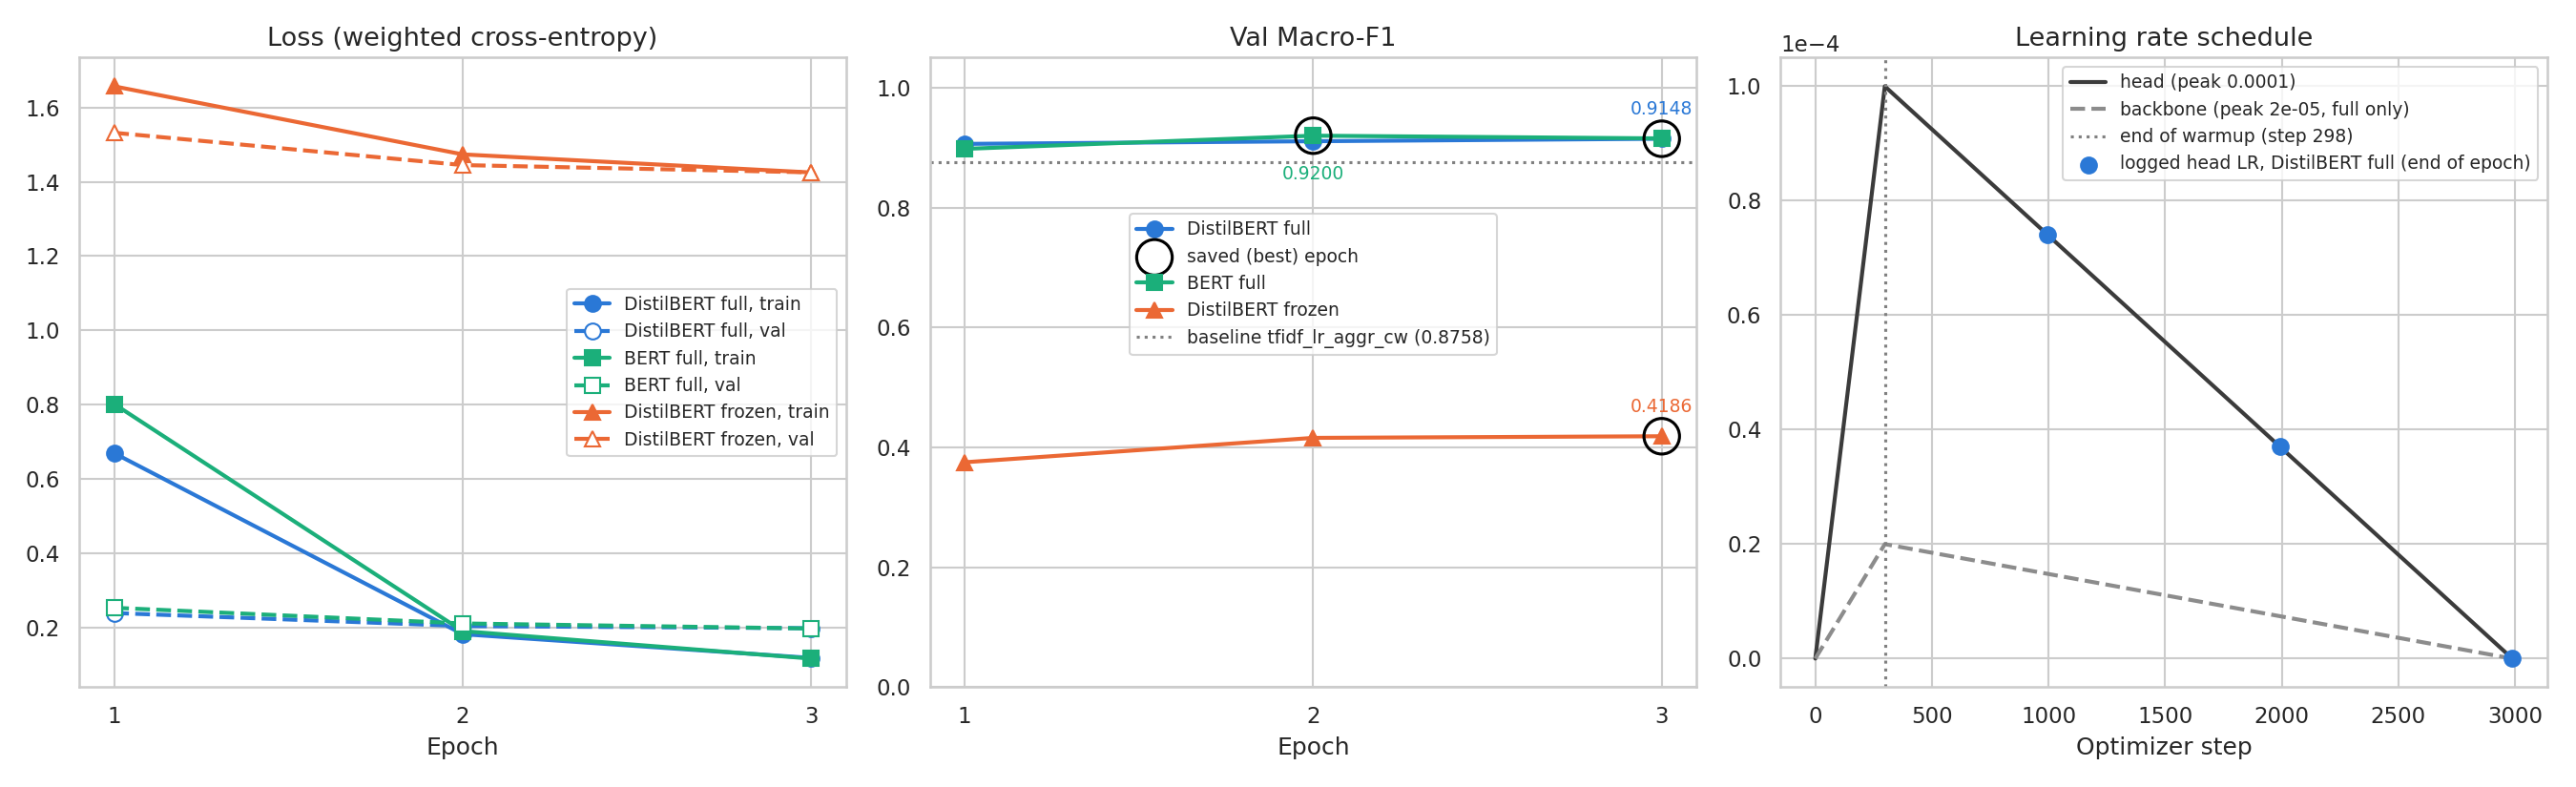
\includegraphics[width=\textwidth]{figures/a2_curves.png}
\caption{Training curves of the seed-42 runs: weighted cross-entropy (left), validation Macro-F1 with the saved epoch circled and the selected baseline as a dotted line (middle), learning rate per step (right). Colour = run (blue DistilBERT, green BERT, orange frozen DistilBERT); in the loss panel solid = training, dashed = validation.}
\label{fig:curves}
\end{figure}

\begin{table}[H]
\centering
\caption{Selected checkpoint (best validation Macro-F1 epoch) of every transformer run.}
\label{tab:ckpt}
\begin{tabular}{@{}lccc@{}}
\toprule
\textbf{Model} & \textbf{Seed 42} & \textbf{Seed 43} & \textbf{Seed 44}\\
\midrule
DistilBERT, full fine-tune & epoch 3 (0.9148) & epoch 3 (0.9178) & epoch 3 (0.9140)\\
BERT, full fine-tune & epoch 2 (0.9200) & epoch 3 (0.9145) & epoch 3 (0.9145)\\
DistilBERT, frozen encoder & epoch 3 (0.4186) & epoch 2 (0.4132) & epoch 3 (0.4253)\\
\bottomrule
\end{tabular}
\end{table}

\paragraph{Implementation issues and fixes.}
\begin{itemize}
  \item The Assignment 1 training function left the first linear layer of the DistilBERT head out of the optimiser; the head is now defined as every parameter outside the encoder, so both head layers are trained.
  \item A first run stopped with a name error because the import cell had not been re-run after adding the padding collator; re-running it fixed the problem.
  \item Single inference timings varied by 10--20\% between runs; timings are now repeated five times after a warm-up and the median is reported (Section~\ref{sec:cost}).
  \item Test metrics are computed after training, so each run's W\&B identifier is stored and the run is resumed to add its test scores.
  \item The whole notebook was rerun from scratch on 8 Nov 2026 with all checkpoints deleted: every validation metric, history and per-class file was identical to the earlier runs; only timings changed.
\end{itemize}

\section{Quantitative Results}

\subsection{Validation (used for every decision)}
\begin{table}[H]
\centering
\caption{Validation results (1,993 texts). Transformers: mean $\pm$ std over seeds 42/43/44.}
\label{tab:val}
\begin{tabular}{@{}llccc@{}}
\toprule
\textbf{Model} & \textbf{Setup} & \textbf{Runs} & \textbf{Accuracy} & \textbf{Macro-F1}\\
\midrule
Majority class (joy) & -- & -- & 0.3522 & 0.0868\\
TF-IDF + LR & minimal text, no class weights & 1 & 0.8289 & 0.7527\\
TF-IDF + LR & minimal text, class weights & 1 & 0.8751 & 0.8489\\
TF-IDF + LR & aggressive text, class weights & 1 & 0.8991 & 0.8758\\
DistilBERT & frozen encoder & 3 & \pmstd{0.4874}{0.0033} & \pmstd{0.4191}{0.0061}\\
DistilBERT & full fine-tune & 3 & \pmstd{0.9373}{0.0005} & \pmstd{0.9155}{0.0020}\\
BERT & full fine-tune & 3 & \pmstd{0.9383}{0.0031} & \pmstd{0.9163}{0.0032}\\
\bottomrule
\end{tabular}
\end{table}

Applying the rules: the aggressive-text baseline (\run{tfidf_lr_aggr_cw}) is the selected baseline (E3); BERT minus DistilBERT is $+0.0008$, smaller than the larger seed std 0.0032, so the two are tied and the smaller model, \textbf{DistilBERT full fine-tune, seed 42} (\run{distil_full_min}), is the final model (E2).

\subsection{Test (evaluated once, after selection)}
\begin{table}[H]
\centering
\caption{Test results (2,000 texts) of all 12 runs.}
\label{tab:test}
\small\setlength{\tabcolsep}{4pt}
\begin{tabular}{@{}lllcccc@{}}
\toprule
\textbf{Model} & \textbf{Setup} & \textbf{Seed} & \textbf{Val F1} & \textbf{Test Acc} & \textbf{Test F1} & \textbf{Test$-$Val}\\
\midrule
\textbf{DistilBERT} & \textbf{full (selected)} & \textbf{42} & \textbf{0.9148} & \textbf{0.9270} & \textbf{0.8902} & $-0.0246$\\
DistilBERT & full & 43 & 0.9178 & 0.9230 & 0.8854 & $-0.0324$\\
DistilBERT & full & 44 & 0.9140 & 0.9245 & 0.8828 & $-0.0313$\\
BERT & full & 42 & 0.9200 & 0.9280 & 0.8881 & $-0.0318$\\
BERT & full & 43 & 0.9145 & 0.9245 & 0.8877 & $-0.0268$\\
BERT & full & 44 & 0.9145 & 0.9270 & 0.8874 & $-0.0271$\\
TF-IDF + LR & aggr., weights (selected) & -- & 0.8758 & 0.8905 & 0.8548 & $-0.0210$\\
TF-IDF + LR & minimal, weights & -- & 0.8489 & 0.8695 & 0.8365 & $-0.0124$\\
TF-IDF + LR & minimal, no weights & -- & 0.7527 & 0.8325 & 0.7289 & $-0.0239$\\
DistilBERT & frozen & 42 & 0.4186 & 0.5010 & 0.4199 & $+0.0013$\\
DistilBERT & frozen & 43 & 0.4132 & 0.4940 & 0.4199 & $+0.0066$\\
DistilBERT & frozen & 44 & 0.4253 & 0.4970 & 0.4233 & $-0.0020$\\
\midrule
Majority class (joy) & -- & -- & 0.0868 & 0.3475 & 0.0860 & --\\
\bottomrule
\end{tabular}
\end{table}

Over seeds, test Macro-F1 is \pmstd{0.8861}{0.0038} for DistilBERT, \pmstd{0.8878}{0.0004} for BERT and \pmstd{0.4210}{0.0020} for the frozen encoder. The selected model gets 1,854 of 2,000 test texts right (146 errors), the selected baseline 1,781 (219 errors). The ranking of all setups is the same on validation and test. The strong models lose 0.02--0.03 Macro-F1 from validation to test; Table~\ref{tab:perclass} shows that this drop comes mostly from surprise (DistilBERT $-0.082$ F1, only 66 test texts) and love ($-0.033$), while sadness and fear barely change. Part of the drop is expected, because the checkpoint epoch and the model were chosen on validation.

\begin{table}[H]
\centering
\caption{Per-class F1 on test (main runs, seed 42) and validation F1 of the selected model.}
\label{tab:perclass}
\begin{tabular}{@{}lrccccc@{}}
\toprule
\textbf{Class} & \textbf{Test texts} & \textbf{Baseline} & \textbf{DistilBERT} & \textbf{BERT} & \textbf{Frozen} & \textbf{DistilBERT val}\\
\midrule
sadness & 581 & 0.9296 & 0.9612 & 0.9643 & 0.5299 & 0.9616\\
joy & 695 & 0.9110 & 0.9504 & 0.9513 & 0.6492 & 0.9561\\
love & 159 & 0.7925 & 0.8523 & 0.8452 & 0.3435 & 0.8853\\
anger & 275 & 0.8917 & 0.9134 & 0.9202 & 0.4329 & 0.9375\\
fear & 224 & 0.8631 & 0.8904 & 0.8825 & 0.4219 & 0.8929\\
surprise & 66 & 0.7407 & 0.7737 & 0.7654 & 0.1421 & 0.8554\\
\midrule
Macro-F1 & 2,000 & 0.8548 & 0.8902 & 0.8881 & 0.4199 & 0.9148\\
\bottomrule
\end{tabular}
\end{table}

\section{Controlled Experiments and Ablation}
\label{sec:exp}
Table~\ref{tab:exp} gives each comparison as A $-$ B in Macro-F1, on validation (where it was decided) and on test (check only).

\begin{table}[H]
\centering
\caption{Experiment results (A $-$ B, Macro-F1). ``A higher'' counts seeds or runs.}
\label{tab:exp}
\small\setlength{\tabcolsep}{4pt}
\begin{tabular}{@{}lcccc@{}}
\toprule
\textbf{Comparison (A $-$ B)} & \textbf{Val mean} & \textbf{Val: A higher} & \textbf{Test mean} & \textbf{Test: A higher}\\
\midrule
E1: full $-$ frozen (DistilBERT) & $+0.4965$ & 3 of 3 & $+0.4651$ & 3 of 3\\
E2: BERT $-$ DistilBERT (full) & $+0.0008$ & 2 of 3 & $+0.0016$ & 2 of 3\\
E3: aggressive $-$ minimal text & $+0.0269$ & 1 of 1 & $+0.0183$ & 1 of 1\\
E4: class weights on $-$ off & $+0.0961$ & 1 of 1 & $+0.1076$ & 1 of 1\\
\bottomrule
\end{tabular}
\end{table}

\paragraph{E1, frozen vs.\ full (main).} Full fine-tuning is higher on all three seeds and the mean gap (0.4965) is far above twice the larger seed std (0.0122): criterion (1) holds. The frozen encoder loses 0.50 Macro-F1, far more than the allowed 0.02, and even scores below the baseline: criterion (2) fails, so it was excluded. The hypothesis is supported. The frozen head has errors spread over all classes (it predicts fear 409 times for 211 true fear texts on validation) and is underfitted (Section~\ref{sec:curves}). It trains in 29\% of the time of full fine-tuning but is \emph{not} faster at inference, since the forward pass is the same. This result holds for this recipe only: the head kept the learning rate and the 3 epochs of full fine-tuning.

\paragraph{E2, BERT vs.\ DistilBERT.} Per seed, BERT $-$ DistilBERT is $+0.0051$, $-0.0033$, $+0.0005$ on validation and $-0.0021$, $+0.0023$, $+0.0047$ on test. Both mean gaps are below the seed std, so the two models are tied; on test, 62 texts are right only for BERT and 60 only for DistilBERT (McNemar exact $p\approx0.93$). The hypothesis of a small gain is not supported at the precision three seeds allow. The changed factor bundles depth, the pretrained pooler and distillation, so the experiment says \emph{whether} BERT differs, not \emph{why}.

\paragraph{E3, stopwords (baseline).} Removing stopwords with the negation keep-list \emph{improved} the baseline on validation ($+0.0269$; F1 higher for all six classes; 85 texts right only with aggressive text vs.\ 37 only with minimal text, McNemar $p\approx2\times10^{-5}$) and on test ($+0.0183$), with half as many n-grams. The hypothesis ``little change'' is therefore rejected. On validation texts with a negation word the accuracy rose from 0.8462 to 0.8910. A likely reason is that removing function words places the negation next to the emotion word, which creates useful bigrams such as ``not happy''. Caveats: one run per setting, untuned TF-IDF and $C$, and the aggressive text also removes non-alphanumeric characters.

\paragraph{E4, class weights (ablation).} Balanced weights raise validation Macro-F1 from 0.7527 to 0.8489 and test Macro-F1 from 0.7289 to 0.8365, much more than accuracy (+0.046 val). As predicted, the small classes gain recall and lose precision (surprise recall 0.40 $\rightarrow$ 0.81, precision 0.89 $\rightarrow$ 0.73 on validation), and F1 improves for all six classes. Weights were therefore used for every later run, transformers included.

\section{Compute Cost}
\label{sec:cost}
Inference was timed with one warm-up and five repeats, keeping the median. Two settings are reported: the whole validation set in batches (baseline on CPU, transformers on the T4 with batches of 16, tokenisation included), and one text at a time for 100 validation texts, which is the only like-for-like comparison of all models on the same CPU (one PyTorch thread).

\begin{table}[H]
\centering
\caption{Cost of the main runs. Training time: mean $\pm$ std over seeds; test Macro-F1: mean over seeds.}
\label{tab:cost}
\small\setlength{\tabcolsep}{4pt}
\begin{tabular}{@{}lrrrrrrc@{}}
\toprule
& & & & \textbf{Batched} & \multicolumn{2}{c}{\textbf{One text (ms)}} & \\
\cmidrule(lr){6-7}
\textbf{Model} & \textbf{Trainable} & \textbf{MB} & \textbf{Train (s)} & \textbf{ms/text} & \textbf{CPU} & \textbf{GPU} & \textbf{Test F1}\\
\midrule
TF-IDF + LR (aggr.) & 102,426 & 1.17 & 5.3 (CPU) & 0.0148 (CPU) & 1.32 & -- & 0.8548\\
DistilBERT full & 66,958,086 & 256.12 & \pmstd{276.9}{10.5} & 1.63 (T4) & 59.64 & 5.92 & 0.8861\\
DistilBERT frozen & 595,206 & 256.12 & \pmstd{81.4}{0.4} & 1.59 (T4) & 60.90 & 4.71 & 0.4210\\
BERT full & 109,486,854 & 418.36 & \pmstd{524.7}{0.5} & 3.16 (T4) & 119.19 & 8.79 & 0.8878\\
\bottomrule
\end{tabular}
\end{table}

Relative to DistilBERT, BERT costs 1.64$\times$ the parameters, 1.89$\times$ the training time and 2.00$\times$ the CPU latency for $+0.0016$ test Macro-F1, a difference within seed noise. The baseline is about 45$\times$ faster than DistilBERT per text on the same CPU and 219$\times$ smaller on disk, for $-0.0314$ mean test Macro-F1 ($-0.0354$ against the selected seed-42 run). GPU memory was not measured, because several models shared the GPU during the run.

\section{Qualitative Results}
Table~\ref{tab:qual} shows test texts that all models get right, difficult texts that only the fine-tuned transformer gets right, and failures. The difficult cases were found by filtering the test predictions for texts with ``but'' or a negation that DistilBERT gets right and the baseline does not; the failures are the random examples (seed 42) printed by the error-analysis cells.

\begin{table}[H]
\centering
\caption{Test texts with the true label and the predictions of the three main models (D = DistilBERT, B = baseline, T = BERT; \checkmark{} = correct).}
\label{tab:qual}
\footnotesize
\begin{tabularx}{\textwidth}{@{}p{1.6cm}Lp{1.3cm}p{1.35cm}p{1.35cm}p{1.35cm}@{}}
\toprule
\textbf{Case} & \textbf{Text} & \textbf{True} & \textbf{D} & \textbf{B} & \textbf{T}\\
\midrule
Easy & im updating my blog because i feel shitty & sadness & \checkmark & \checkmark & \checkmark\\
Easy & i felt anger when at the end of a telephone call & anger & \checkmark & \checkmark & \checkmark\\
Easy & i find myself in the odd position of feeling supportive of & love & \checkmark & \checkmark & \checkmark\\
\midrule
Difficult, correct & i was feeling pretty anxious all day but my first day at work was a very good day and that helped a lot & fear & \checkmark{} (1.00) & joy & \checkmark\\
Difficult, correct & i do feel welcomed but it s a little weird & joy & \checkmark{} (1.00) & surprise & \checkmark\\
Difficult, correct & i just feel extremely comfortable with the group of people that i dont even need to hide myself & joy & \checkmark{} (1.00) & anger & \checkmark\\
\midrule
Failure (G1) & i chant the invocation and feel his force supporting me as i teach & joy & love (0.63) & love & \checkmark\\
Failure (G2) & when i learnt that my best friend had failed the exams & anger & sadness (0.88) & \checkmark & sadness\\
Failure (G3) & i started to feel so overwhelmed & fear & surprise (0.70) & surprise & surprise\\
Failure (G5) & i feel accepted and loved by a community of derby girls that i helped to create & joy & love (0.90) & love & love\\
\bottomrule
\end{tabularx}
\end{table}

The transformer handles texts where the emotion word is contrasted or softened (``anxious \ldots{} but \ldots{} a very good day'' is still labelled fear). The baseline follows the words with the largest weights (``good'', ``weird''). The failures involve close emotions, and in the last example all three models agree on a label (love) that is arguably as plausible as the gold label (joy).

\section{Error Analysis}
\label{sec:errors}
The analysis covers the 146 test errors of the selected model and compares them with the baseline (219 errors) and BERT (144 errors) on the same texts. The model predictions come from the single test evaluation; nothing was re-run.

\subsection{Confusion Pairs}
\begin{table}[H]
\centering
\caption{Largest true $\rightarrow$ predicted confusions on test (ordered by DistilBERT). The last column is the share of the true class that DistilBERT sends to that label.}
\label{tab:pairs}
\begin{tabular}{@{}llrrrr@{}}
\toprule
\textbf{True} & \textbf{Predicted} & \textbf{DistilBERT} & \textbf{Baseline} & \textbf{BERT} & \textbf{\% of true class}\\
\midrule
joy & love & 42 & 58 & 20 & 6.04\\
anger & sadness & 12 & 8 & 17 & 4.36\\
anger & fear & 12 & 7 & 7 & 4.36\\
fear & surprise & 11 & 19 & 26 & 4.91\\
sadness & anger & 11 & 23 & 5 & 1.89\\
surprise & fear & 10 & 2 & 0 & 15.15\\
joy & surprise & 7 & 11 & 7 & 1.01\\
love & joy & 6 & 8 & 28 & 3.77\\
sadness & fear & 6 & 8 & 2 & 1.03\\
fear & sadness & 6 & 8 & 5 & 2.68\\
\bottomrule
\end{tabular}
\end{table}

The errors are concentrated: the three largest pairs hold 66 of the 146 errors (45.2\%), and every listed pair links two close emotions; no pair links opposite emotions such as joy and anger. In absolute numbers joy $\rightarrow$ love is the largest error, but relative to class size the worst case is surprise $\rightarrow$ fear (15\% of all surprise texts), which explains the low surprise F1. The \emph{direction} of an error shows a model's bias: DistilBERT pushes joy towards love (42 vs.\ 6 the other way), while BERT pushes love towards joy (28 vs.\ 20) and over-predicts surprise (fear $\rightarrow$ surprise 26, never surprise $\rightarrow$ fear; surprise precision 0.65, recall 0.94).

\subsection{Error Groups}
The pairs are merged into groups that share a hypothesised cause; G1--G3 and ``other'' partition the errors, so each error is counted once.

\begin{table}[H]
\centering
\caption{Error groups on test: number of errors (share of the model's errors), hypothesised cause and possible improvement.}
\label{tab:groups}
\footnotesize
\begin{tabularx}{\textwidth}{@{}p{2.2cm}ccc LL@{}}
\toprule
\textbf{Group} & \textbf{DistilBERT} & \textbf{Baseline} & \textbf{BERT} & \textbf{Hypothesised cause} & \textbf{Possible improvement}\\
\midrule
G1 joy $\leftrightarrow$ love & 48 (32.9\%) & 66 (30.1\%) & 48 (33.3\%) & Love texts often describe a happy feeling about someone, so the classes share words; class weights (love 2.07 vs.\ joy 0.50) push ambiguous texts to love & More love examples; per-class decision thresholds tuned on validation\\
\addlinespace
G2 sadness / anger / fear & 51 (34.9\%) & 61 (27.9\%) & 45 (31.2\%) & One negative word (hurt, upset, stressed) fits several negative emotions; one text can hold more than one emotion & Multi-label annotation; use more context than the single emotion word\\
\addlinespace
G3 fear $\leftrightarrow$ surprise & 21 (14.4\%) & 21 (9.6\%) & 26 (18.1\%) & Surprise is the smallest class (564 training texts) and shares words such as ``overwhelmed'', ``shocked'' with fear & More surprise data or augmentation; a surprise threshold tuned on validation\\
\addlinespace
Other pairs & 26 (17.8\%) & 71 (32.4\%) & 25 (17.4\%) & Scattered errors, mostly keyword-driven for the baseline & --\\
\bottomrule
\end{tabularx}
\end{table}

The transformers remove most of the baseline's scattered errors (``other'' falls from 71 to 26) but not the three structural groups: G1 has the same size for both transformers, only with opposite directions, which suggests that the joy/love boundary is unclear in the labels themselves rather than a weakness of one model.

\subsection{Label Noise and Text Properties}
\textbf{Possible label noise.} On 50 test texts all three models give the same wrong label; they make up 34.2\% of DistilBERT's errors. Three different models agreeing against the gold label points to a doubtful label or a truly ambiguous text. The 14 test texts whose copy in train or validation had another label (removed by filtering) support this: DistilBERT gets only 5 of them right, and on all 9 others it predicts exactly the label of the removed copy, e.g.\ ``i feel like i am in paradise kissing those sweet lips make me feel like i dive into a magical world of love'' is labelled joy in test and love in its training copy, and DistilBERT predicts love.

\textbf{Where context helps.} The advantage of DistilBERT over the baseline is largest on long texts ($\ge$ 35 words: accuracy 0.920 vs.\ 0.806), texts with ``but'' (0.929 vs.\ 0.854) and texts with a negation word (0.912 vs.\ 0.857), and smallest on short texts ($\le$ 11 words: 0.943 vs.\ 0.924). The model is also overconfident when wrong: mean confidence 0.985 on correct and 0.796 on wrong predictions, with 47 of the 146 errors above 0.9.

\begin{figure}[H]
\centering
\begin{subfigure}{0.48\textwidth}\centering
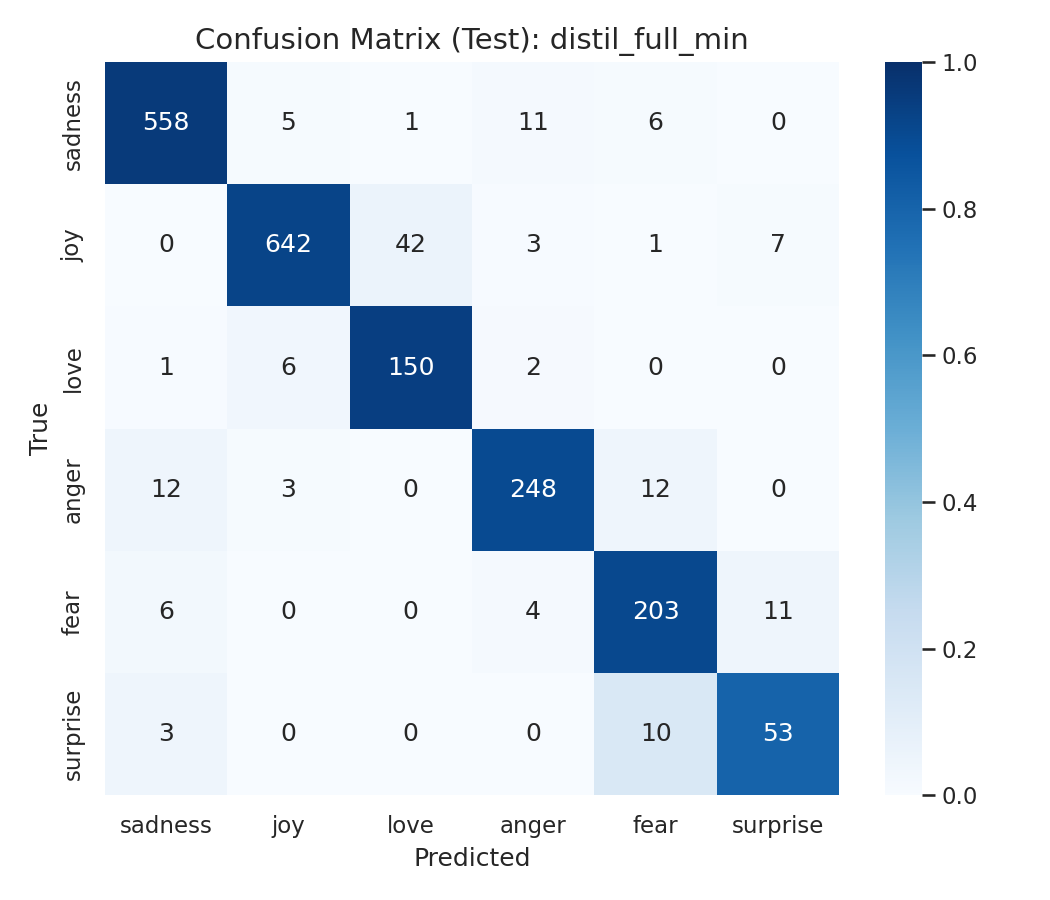
\includegraphics[width=\linewidth]{figures/a2_cm_test_distil_full_min.png}
\caption{DistilBERT full fine-tune (selected), test Macro-F1 0.8902}
\end{subfigure}\hfill
\begin{subfigure}{0.48\textwidth}\centering
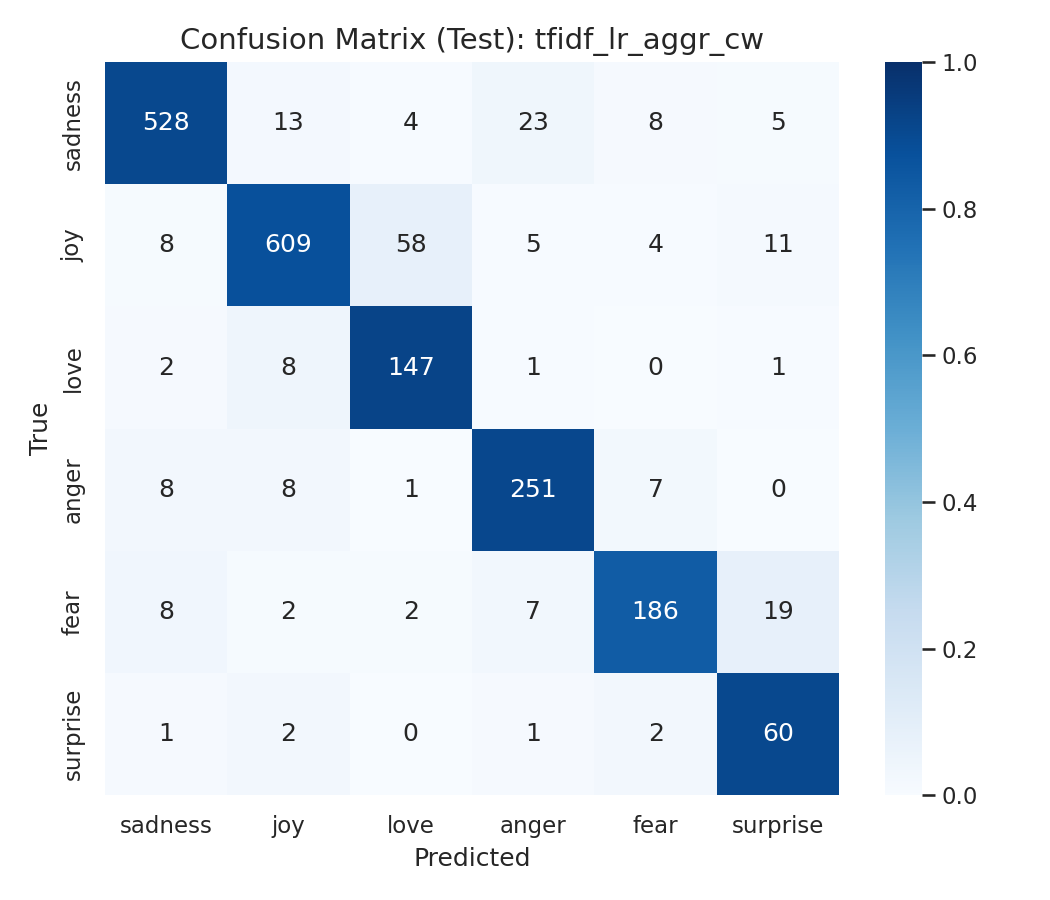
\includegraphics[width=\linewidth]{figures/a2_cm_test_tfidf_lr_aggr_cw.png}
\caption{TF-IDF + LR, aggressive text (selected baseline), 0.8548}
\end{subfigure}\\[4pt]
\begin{subfigure}{0.48\textwidth}\centering
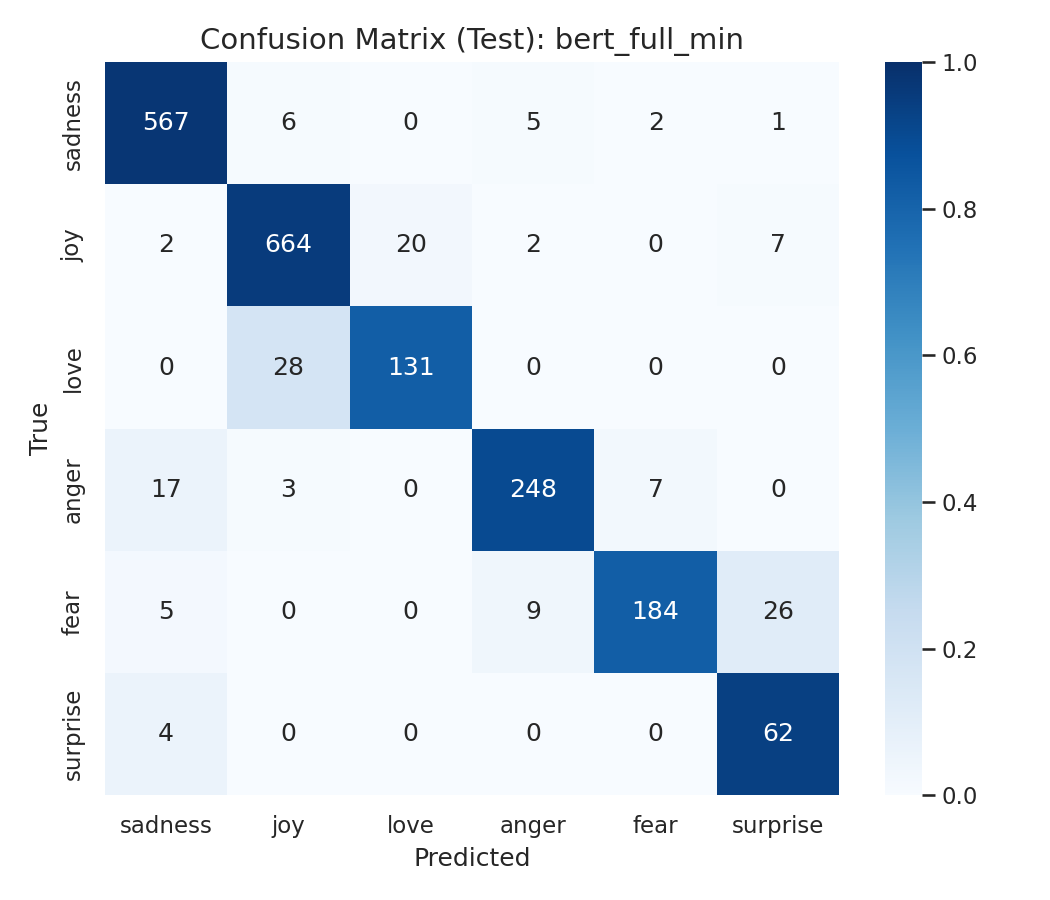
\includegraphics[width=\linewidth]{figures/a2_cm_test_bert_full_min.png}
\caption{BERT full fine-tune, 0.8881}
\end{subfigure}\hfill
\begin{subfigure}{0.48\textwidth}\centering
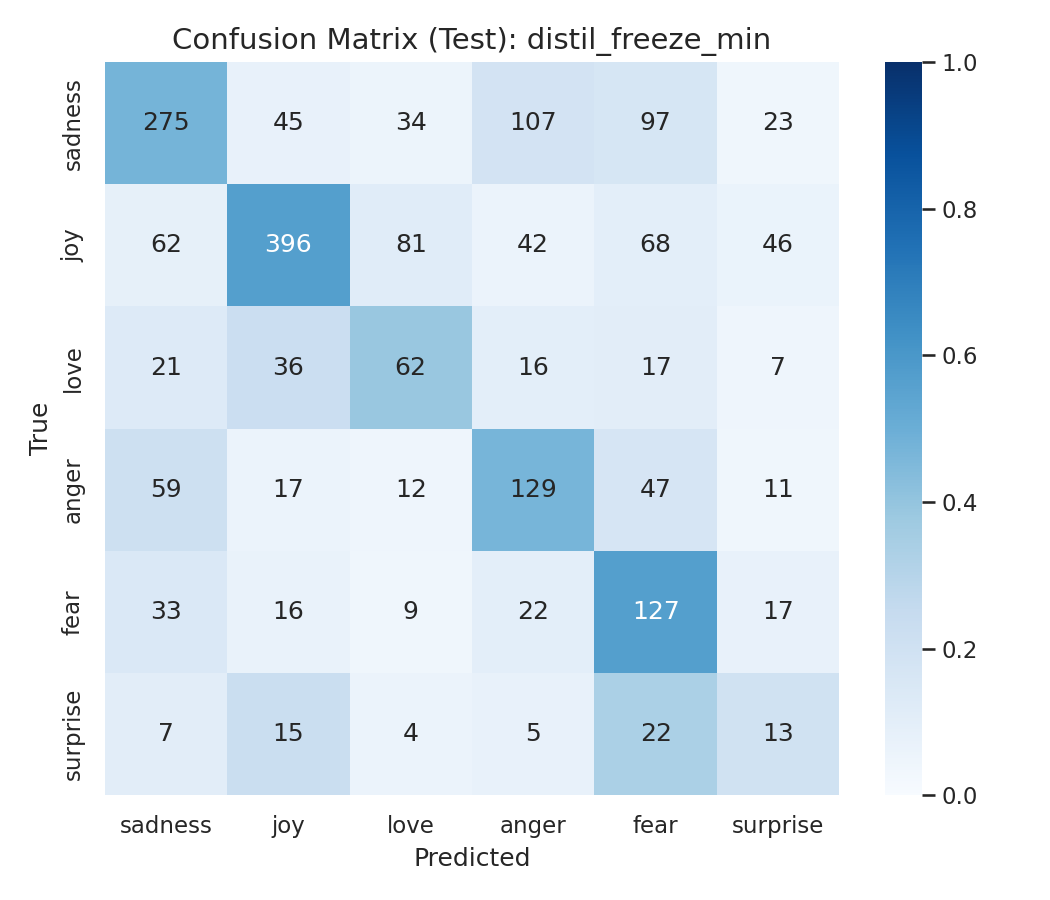
\includegraphics[width=\linewidth]{figures/a2_cm_test_distil_freeze_min.png}
\caption{DistilBERT frozen encoder, 0.4199}
\end{subfigure}
\caption{Test confusion matrices of the seed-42 main runs.}
\label{fig:cm}
\end{figure}

\section{Comparison and Discussion}
\begin{enumerate}
  \item \textbf{Fine-tuning beats the baseline, by a clear but moderate margin.} DistilBERT exceeds the selected baseline by $+0.0354$ test Macro-F1 and $+0.0365$ accuracy, improves all six classes (most for love, $+0.060$ F1), and the difference is not chance: 124 texts are right only for DistilBERT, 51 only for the baseline (McNemar exact $p\approx3\times10^{-8}$). The gain comes from texts where one emotion word is not enough (long, contrastive or negated texts); on short texts the baseline is almost as good, which agrees with the EDA finding that most labels follow a single emotion word.
  \item \textbf{A bigger encoder does not help here.} BERT and DistilBERT are tied on validation and test and make the same number of errors in each group, while BERT costs about twice as much. On this dataset the bottleneck appears to be the labels and the close classes, not model capacity.
  \item \textbf{The encoder must be adapted.} With a frozen encoder the model is worse than a bag of n-grams. The \texttt{[CLS]} vector of a model pre-trained with masked-language modelling does not linearly separate these emotions, and the recipe gives the head too few effective updates. Freezing saves training time only, not inference time.
  \item \textbf{Simple choices matter for the baseline.} Class weights (+0.108 test Macro-F1) and stopword removal with a negation keep-list (+0.018) together move the baseline from 0.7289 to 0.8548, closing much of the gap to the transformer at a tiny fraction of its cost.
  \item \textbf{Trade-off.} If CPU latency or memory matters (1.3 ms vs.\ 60 ms per text, 1 MB vs.\ 256 MB) the improved baseline is a reasonable choice; if quality on harder texts matters, DistilBERT is the best quality per cost; BERT is not worth its extra cost here.
  \item \textbf{What cannot be concluded.} The ranking of BERT and DistilBERT; whether a frozen encoder would work with a tuned learning rate or more epochs; whether the stopword gain holds for tuned TF-IDF settings; and the absolute scores without hyperparameter search. Three seeds give only a rough estimate of the spread.
\end{enumerate}

\section{Limitations and Conclusion}
\paragraph{Limitations.}
\begin{itemize}
  \item \textbf{Data:} one English dataset of short, informal texts with machine-generated labels; conflicting duplicates show label noise, 14 test texts carry disputed labels, and near-duplicates (texts differing by a few words) were not audited. The test set is small for surprise (66 texts), so its F1 moves by about 0.015 per error.
  \item \textbf{Method:} no hyperparameter search for any model; the frozen-encoder result holds for one recipe; no per-class thresholds; single-label output although some texts express several emotions.
  \item \textbf{Experiments:} three seeds per transformer and a single run per baseline setting; timings come from a shared Colab machine (one CPU thread, one T4) and GPU memory was not measured.
\end{itemize}

\paragraph{Conclusion.} \emph{Research question: does fine-tuning a pretrained Transformer beat a classical TF-IDF baseline on six-class emotion classification, and at what cost?} Yes: fully fine-tuned DistilBERT reaches test Macro-F1 0.8902 (accuracy 0.9270) against 0.8548 for the best baseline, with gains on every class and mostly on texts that need context, at about 45 times the CPU latency and 650 times the parameters. BERT gives no measurable improvement for twice the cost, and freezing the encoder does not work under the same recipe. The remaining errors lie between close emotions and partly reflect doubtful labels.

\paragraph{Future work.} Tune per-class thresholds on validation for love and surprise; clean or re-annotate the conflicting and all-models-wrong texts, or move to multi-label targets; tune the learning rate and the number of epochs of the frozen head; and shrink DistilBERT for CPU use (quantisation or further distillation).

\section{Reproducibility}
\begin{itemize}
  \item \textbf{Code:} \texttt{notebooks/A2\_emotion.ipynb} in the repository, run top to bottom on a Colab T4 (``Run all''); the full run from scratch takes about 45 minutes. The repository README gives installation, data preparation, training and evaluation steps.
  \item \textbf{Configuration:} one configuration cell holds every setting; the exported configuration file, hardware file and all result tables are in the \texttt{results/} folder of the repository.
  \item \textbf{Data and seeds:} dataset revision pinned; seeds 42, 43, 44; the training batch order depends only on the seed.
  \item \textbf{Checkpoints:} each run keeps its best-validation epoch on Google Drive; the whole Drive folder is shared (link on the title page): all 12 checkpoints in \texttt{A2/checkpoints/} (one sub-folder per transformer run, one \texttt{.joblib} file per baseline) and the selected DistilBERT model with the selected baseline as one archive, \texttt{A2/checkpoints\_final.zip} (257.3 MB). The repository README explains how to download a run and load it. A loading switch reuses saved checkpoints instead of retraining; turning it off rebuilds all 12 runs.
  \item \textbf{Experiment logs:} every reported number is traceable to a W\&B run (Table~\ref{tab:wandb}); each run stores its configuration, per-epoch curves and, in its summary, the test scores.
  \item \textbf{Commit:} tag \href{https://github.com/volethanhtrieu/DL_Assignment-02/tree/a2-final}{\texttt{a2-final}}, the final commit of Assignment 02 on the \texttt{main} branch (submitted 11 Nov 2026).
\end{itemize}

\begin{table}[H]
\centering
\caption{W\&B run identifiers (project \texttt{goat-a2-emotion}).}
\label{tab:wandb}
\small
\begin{tabular}{@{}llll@{}}
\toprule
\textbf{Run} & \textbf{ID} & \textbf{Run} & \textbf{ID}\\
\midrule
\run{tfidf_lr_min_nocw} & 7wlsxtx8 & \run{bert_full_min} & ulss79nz\\
\run{tfidf_lr_min_cw} & pwfi016q & \run{bert_full_min_s43} & pil00scg\\
\run{tfidf_lr_aggr_cw} & 3ojjzuey & \run{bert_full_min_s44} & noxjos1c\\
\run{distil_full_min} & lnuy747a & \run{distil_freeze_min} & 7rugvdvg\\
\run{distil_full_min_s43} & psflj88c & \run{distil_freeze_min_s43} & 83s806pr\\
\run{distil_full_min_s44} & llw3bte9 & \run{distil_freeze_min_s44} & k1uomhhg\\
\bottomrule
\end{tabular}
\end{table}

The public project holds these 12 runs plus one run that is not used anywhere (\texttt{x3xl0d1a}, one epoch, no test scores): the start of the final rerun, stopped and restarted. In each run summary, \emph{val\_macro\_f1} is the value of the \emph{last} epoch; the saved (best) epoch can differ (BERT seed 42 and frozen seed 43, Table~\ref{tab:ckpt}), so selected scores are those of Table~\ref{tab:ckpt} and the test scores in the summaries.

% =====================================================================
\section{AI Usage Disclosure}
% =====================================================================
Following handbook \S5, Table~\ref{tab:ai} records the one AI tool used in this assignment. The detailed log is \texttt{AI\_USAGE.md} in the repository.

\begin{table}[H]
\centering
\caption{AI usage disclosure (handbook \S5.2 mandatory fields).}
\label{tab:ai}
\footnotesize
\begin{tabularx}{\textwidth}{@{}p{3.3cm}L@{}}
\toprule
\textbf{Field} & \textbf{Disclosure}\\
\midrule
1. Tool and model & Claude Code (Anthropic), model Claude Opus 5.5 (one session on Claude Sonnet 5.5, 25 Oct 2026)\\
2. Member who used it & Võ Lê Thành Triệu\\
3. Time / stage & 25--28 Oct 2026 (M2: EDA, filtering, baseline, DistilBERT and BERT, preliminary results, report page) and 4--11 Nov 2026 (M3: controlled experiments, test evaluation, error analysis, compute cost, export, checkpoints section, Hugging Face model repository and live demo, this report, presentation slides and video script)\\
4. Purpose & experiment-design advice, coding assistance, debugging, result checking and analysis, concept explanation, web page design and report drafting (including the LaTeX source of this report), deployment of the selected models to Hugging Face (model repository and in-browser demo), slide generation and video-script drafting\\
5. Affected sections & the notebook (all blocks), the assignment page, README, Sections 1--17 of this report, the Hugging Face model repository and demo (\texttt{hf\_space/}), the presentation slides and the video script\\
6. Representative prompts & ``Write block 8: apply filtering rules 1--4 from proposal \S5 \ldots{} assert no overlap, $\ge$ 5,000 train rows and 6 classes per split.'' --- ``Write blocks 25 and 26: repeated inference timing, cost table and full export.'' --- ``Write the LaTeX report from the files in results/ only, following the handbook and our template; no code in the report.'' --- ``create slide for presentation for me include with crucial number and table for me, keep layout clean, include graph in results''\\
7. How the output was edited and verified & every cell was read, run on Colab and explained by the member before it was kept; key numbers (split sizes, class weights, Macro-F1, seed means, McNemar counts, error-group counts) were recomputed from the exported CSV files; every number in this report was traced to \texttt{results/} or the run notebook; the text was read and edited by the member; the slides were read again and every number on them checked against \texttt{results/} and this report, and the video script was read again and rewritten by the member in their own words; the models converted for the demo gave the same prediction as the original checkpoints on all 2,000 test texts\\
8. Responsible member & Võ Lê Thành Triệu\\
9. Verification sources & the course handbook; documentation of scikit-learn, PyTorch, Hugging Face transformers, datasets, Hub and transformers.js, W\&B; the papers in the references; the Colab outputs\\
\midrule
Not used for & creating data, metrics, examples or results; all decisions (filtering rules, class weights tested on validation, the experiments and the freeze threshold of 0.02, adding BERT and 3 seeds, model selection rules fixed before any test result, final baseline, short form of the error analysis) were made by Võ Lê Thành Triệu; the AI suggested options and made no decisions\\
\bottomrule
\end{tabularx}
\end{table}

\subsection{Declaration}
I, \textbf{Võ Lê Thành Triệu} (2453297), declare that: (1) I carried out Assignment 02 and take responsibility for all code, numbers, figures and text in this submission; (2) the AI tool above was used as an assistant under my review, and I can explain every part of the work; (3) no data, result, checkpoint, parameter count or reference was fabricated --- every number comes from runs I executed on Google Colab; (4) the test set was used only after model selection.

\vspace{0.4cm}
\noindent\textbf{Signature:} \emph{Võ Lê Thành Triệu} \hfill \textbf{Date:} 11 November 2026

% =====================================================================
\begin{thebibliography}{99}
\bibitem{saravia2018} E.~Saravia, H.-C.~T.~Liu, Y.-H.~Huang, J.~Wu, and Y.-S.~Chen, ``CARER: Contextualized affect representations for emotion recognition,'' in \emph{Proc. EMNLP}, 2018, pp.~3687--3697. doi:~\href{https://doi.org/10.18653/v1/D18-1404}{10.18653/v1/D18-1404}. Dataset: \url{https://huggingface.co/datasets/dair-ai/emotion}
\bibitem{salton1988} G.~Salton and C.~Buckley, ``Term-weighting approaches in automatic text retrieval,'' \emph{Information Processing \& Management}, vol.~24, no.~5, pp.~513--523, 1988. doi:~\href{https://doi.org/10.1016/0306-4573(88)90021-0}{10.1016/0306-4573(88)90021-0}
\bibitem{vaswani2017} A.~Vaswani \emph{et al.}, ``Attention is all you need,'' in \emph{Advances in NeurIPS}, 2017. \url{https://arxiv.org/abs/1706.03762}
\bibitem{devlin2019} J.~Devlin, M.-W.~Chang, K.~Lee, and K.~Toutanova, ``BERT: Pre-training of deep bidirectional transformers for language understanding,'' in \emph{Proc. NAACL-HLT}, 2019, pp.~4171--4186. doi:~\href{https://doi.org/10.18653/v1/N19-1423}{10.18653/v1/N19-1423}
\bibitem{sanh2019} V.~Sanh, L.~Debut, J.~Chaumond, and T.~Wolf, ``DistilBERT, a distilled version of BERT: smaller, faster, cheaper and lighter,'' \emph{arXiv:1910.01108}, 2019. \url{https://arxiv.org/abs/1910.01108}
\bibitem{loshchilov2019} I.~Loshchilov and F.~Hutter, ``Decoupled weight decay regularization,'' in \emph{Proc. ICLR}, 2019. \url{https://arxiv.org/abs/1711.05101}
\bibitem{wolf2020} T.~Wolf \emph{et al.}, ``Transformers: State-of-the-art natural language processing,'' in \emph{Proc. EMNLP: System Demonstrations}, 2020, pp.~38--45. doi:~\href{https://doi.org/10.18653/v1/2020.emnlp-demos.6}{10.18653/v1/2020.emnlp-demos.6}
\bibitem{paszke2019} A.~Paszke \emph{et al.}, ``PyTorch: An imperative style, high-performance deep learning library,'' in \emph{Advances in NeurIPS}, 2019. \url{https://arxiv.org/abs/1912.01703}
\bibitem{pedregosa2011} F.~Pedregosa \emph{et al.}, ``Scikit-learn: Machine learning in Python,'' \emph{J. Mach. Learn. Res.}, vol.~12, pp.~2825--2830, 2011. \url{https://jmlr.org/papers/v12/pedregosa11a.html}
\bibitem{mcnemar1947} Q.~McNemar, ``Note on the sampling error of the difference between correlated proportions or percentages,'' \emph{Psychometrika}, vol.~12, no.~2, pp.~153--157, 1947. doi:~\href{https://doi.org/10.1007/BF02295996}{10.1007/BF02295996}
\bibitem{wandb} L.~Biewald, ``Experiment tracking with Weights and Biases,'' 2020. Software available from \url{https://wandb.ai}
\end{thebibliography}

\end{document}
